\captionsetup[figure]{font=footnotesize,labelfont=footnotesize}

\section{Yearbook -- Drift Matrices}
\label{app:yearbook}

\noindent The cohort-mean and per-model deviation matrices shown here, and the in-distribution, future, and decay quantities tabulated below, are defined in Section~\ref{subsec:drift_summary}.

\begin{figure}[H]
\centering
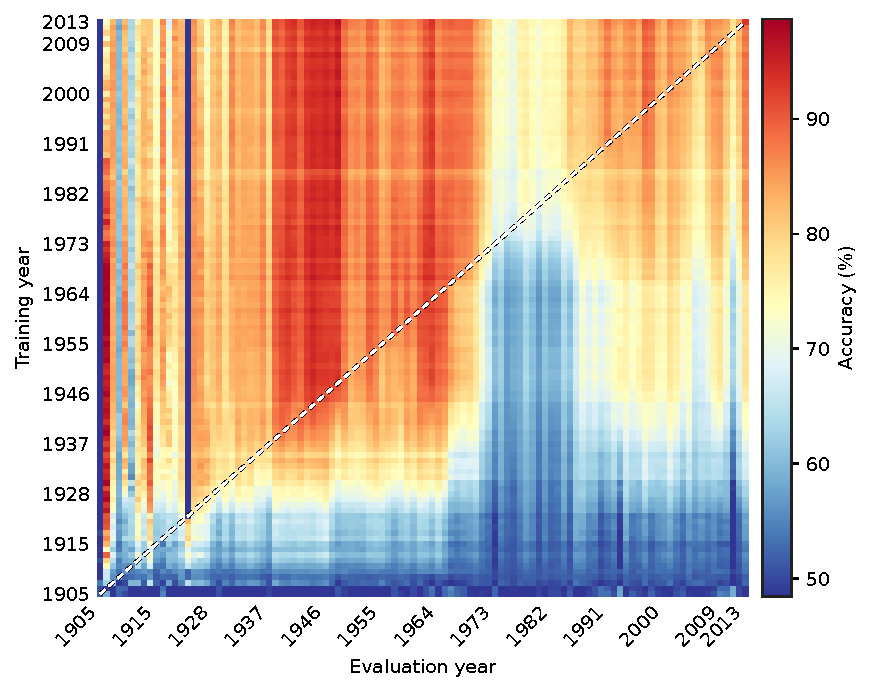
\includegraphics[width=0.5\textwidth]{plots_experiments/yearbook/mean_accuracy_matrix.pdf}
\caption{Cohort-mean Accuracy matrix $\bar{M}$ over the Yearbook models. Cell $(i,j)$ is the mean across those models of the score from training through slice $i$ and evaluating on slice $j$.}
\label{fig:yearbook_mean_matrix}
\end{figure}

\subsection{Model Roster}

\noindent
\begin{minipage}[t]{0.49\linewidth}
\centering
\footnotesize
\captionof{table}{Yearbook: models trained from scratch.}
\label{tab:yearbook_roster}
\resizebox{\ifdim\width>\linewidth \linewidth\else\width\fi}{!}{%
\begin{tabular}{l l r}
\toprule
Model & Family & Parameters \\
\midrule
ViT-S & ViT & 75k \\
CNN-S & CNN & 94k \\
ResNet-S & ResNet & 98k \\
MLP-S & MLP & 98k \\
ResNet-M & ResNet & 400k \\
MLP-M & MLP & 410k \\
CNN-M & CNN & 542k \\
ViT-M & ViT & 545k \\
MLP-L & MLP & 2.1M \\
ResNet-L & ResNet & 2.1M \\
CNN-L & CNN & 2.1M \\
ViT-L & ViT & 2.2M \\
\bottomrule
\end{tabular}}
\end{minipage}
\hfill
\begin{minipage}[t]{0.49\linewidth}
\centering
\footnotesize
\captionof{table}{Yearbook: frozen pretrained encoders, with trainable head and total parameters.}
\label{tab:yearbook_roster_frozen}
\resizebox{\ifdim\width>\linewidth \linewidth\else\width\fi}{!}{%
\begin{tabular}{l l rr}
\toprule
Model & Family & Trainable & Total \\
\midrule
DINOv3-S & Transfer & 770 & 21.6M \\
ViT-S16-IN21k & Transfer & 770 & 21.7M \\
DINOv2-S & Transfer & 770 & 22.1M \\
ResNet50-IN & Transfer & 4k & 23.5M \\
ConvNeXt-S & Transfer & 2k & 49.5M \\
EVA02-B & Transfer & 2k & 85.8M \\
MAE-B & Transfer & 2k & 85.8M \\
CLIP-B32 & Transfer & 2k & 87.5M \\
SigLIP-B & Transfer & 2k & 92.9M \\
\bottomrule
\end{tabular}}
\end{minipage}


\subsection{MLP}

\begin{figure}[H]
\centering
\begin{subfigure}[t]{0.49\textwidth}\centering
    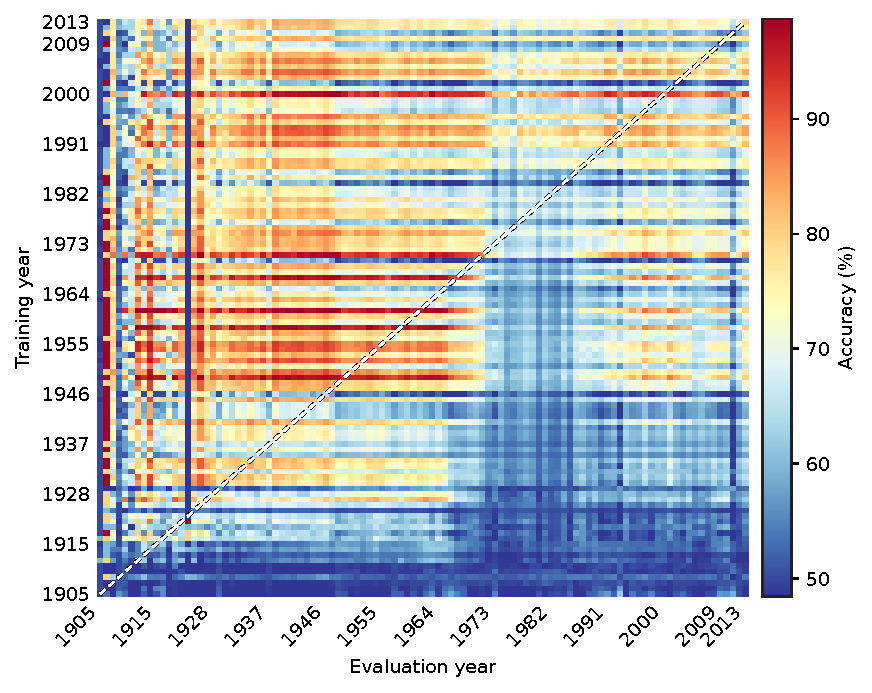
\includegraphics[width=0.49\linewidth]{plots_experiments/yearbook/raw/MLP-S_drift_matrix.pdf}\hfill
    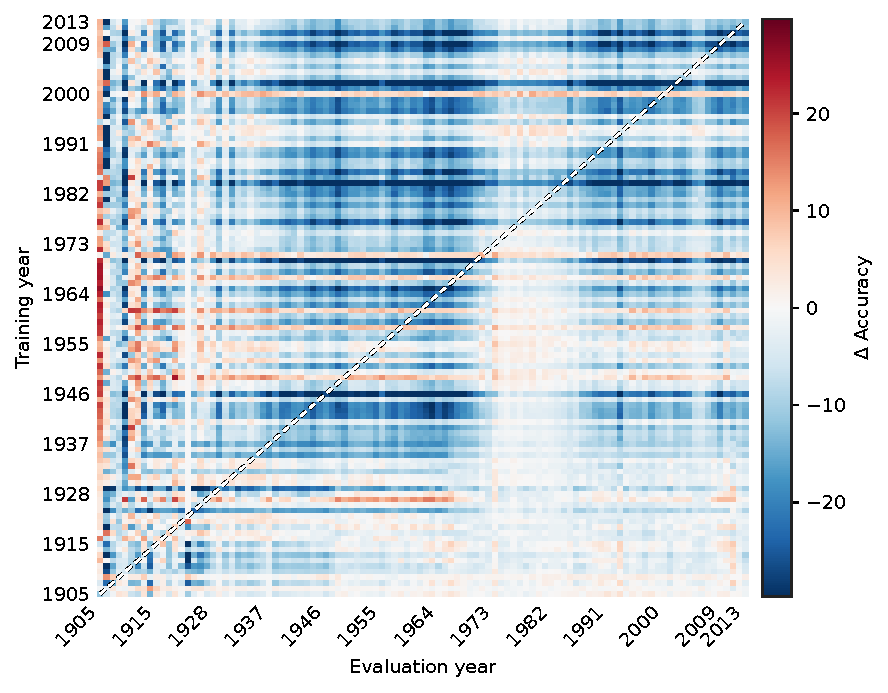
\includegraphics[width=0.49\linewidth]{plots_experiments/yearbook/deviation/MLP-S_deviation.pdf}
    \caption{MLP-S}
    \label{fig:yearbook_MLP_S}
\end{subfigure}
\hfill
\begin{subfigure}[t]{0.49\textwidth}\centering
    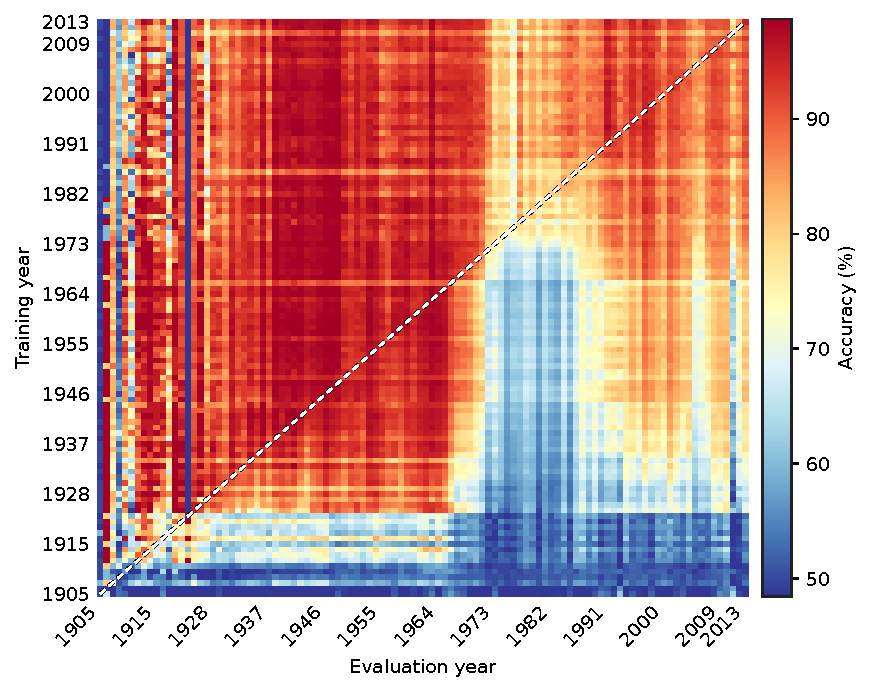
\includegraphics[width=0.49\linewidth]{plots_experiments/yearbook/raw/MLP-M_drift_matrix.pdf}\hfill
    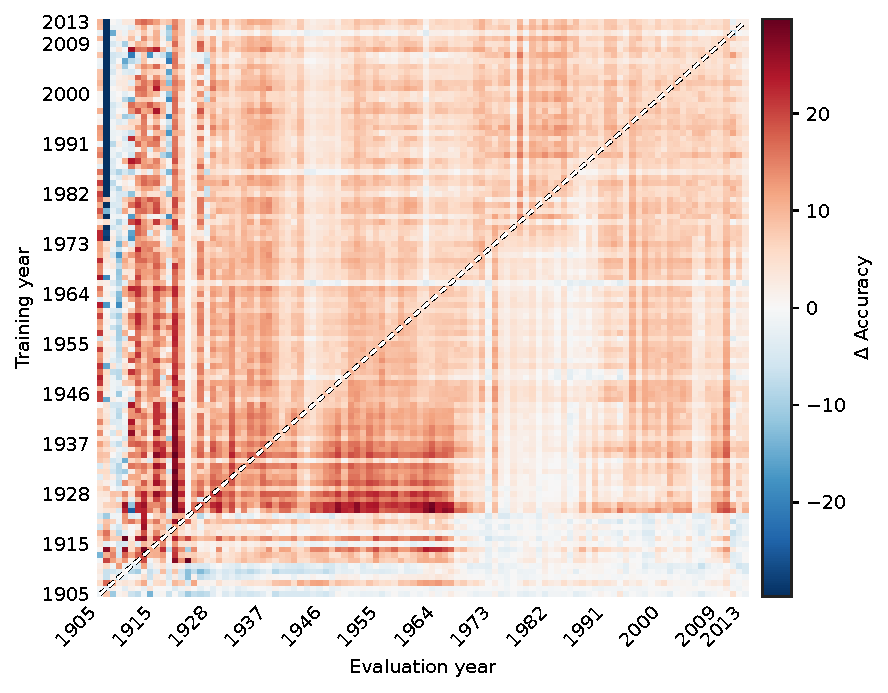
\includegraphics[width=0.49\linewidth]{plots_experiments/yearbook/deviation/MLP-M_deviation.pdf}
    \caption{MLP-M}
    \label{fig:yearbook_MLP_M}
\end{subfigure}

\begin{subfigure}[t]{0.49\textwidth}\centering
    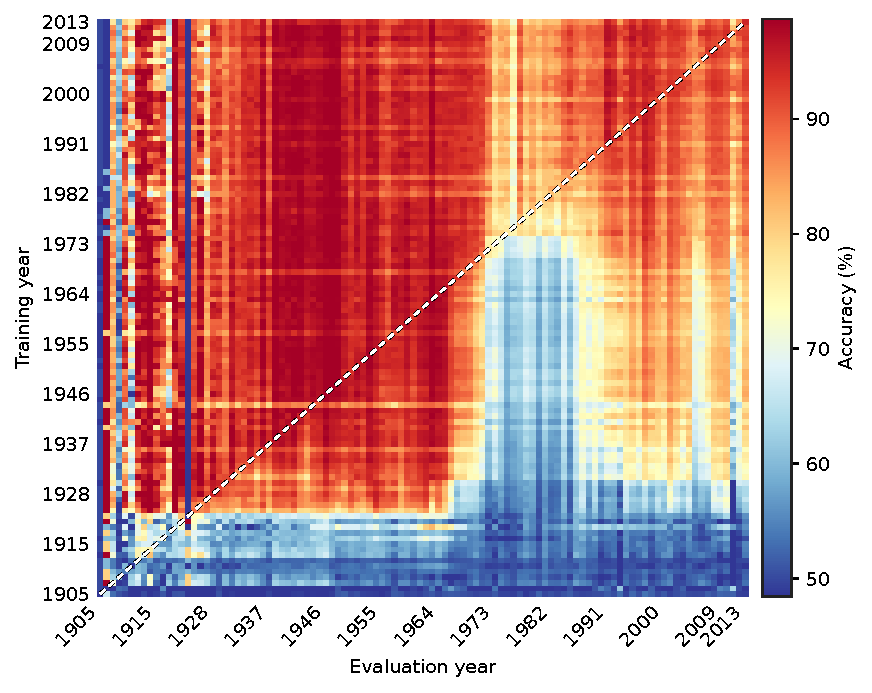
\includegraphics[width=0.49\linewidth]{plots_experiments/yearbook/raw/MLP-L_drift_matrix.pdf}\hfill
    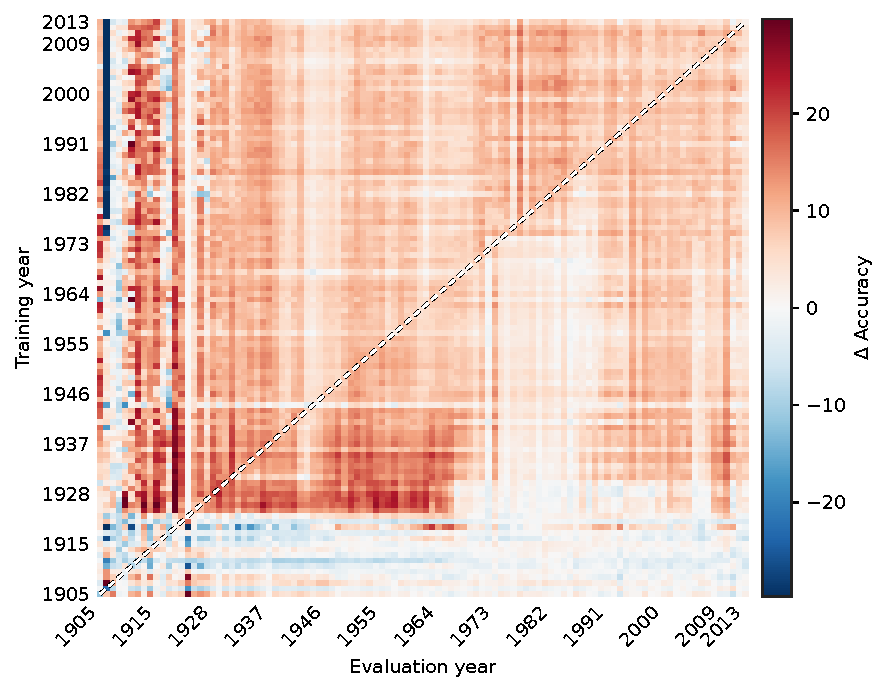
\includegraphics[width=0.49\linewidth]{plots_experiments/yearbook/deviation/MLP-L_deviation.pdf}
    \caption{MLP-L}
    \label{fig:yearbook_MLP_L}
\end{subfigure}
\caption{MLP models: Accuracy drift matrix $M^{(m)}$ and deviation from the cohort mean $\Delta^{(m)} = M^{(m)} - \bar{M}$ for each model, shown on a sequential and a zero-centred diverging scale, respectively.}
\label{fig:yearbook_family_image_mlp}
\end{figure}

\subsection{CNN}

\begin{figure}[H]
\centering
\begin{subfigure}[t]{0.49\textwidth}\centering
    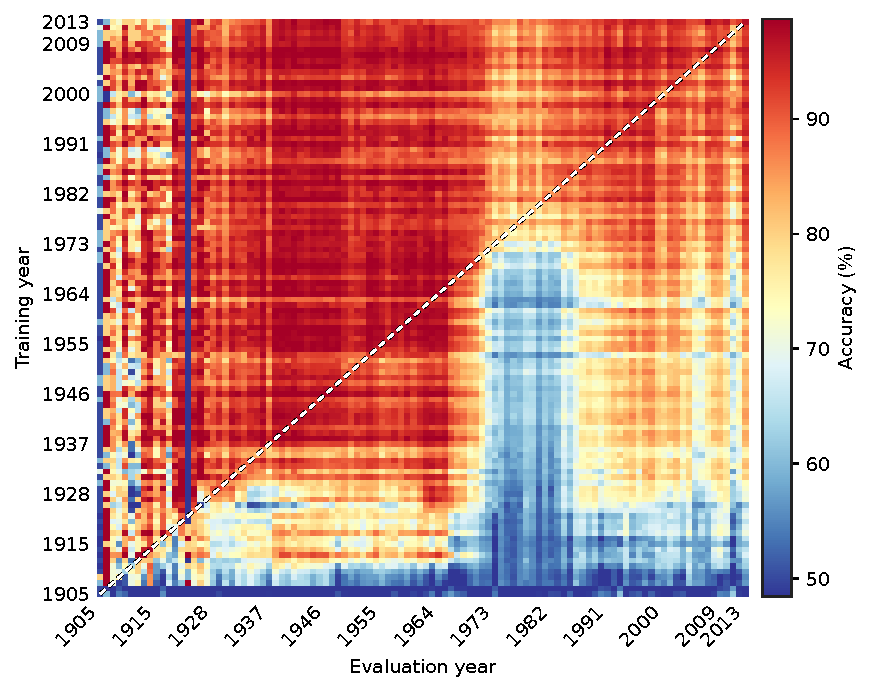
\includegraphics[width=0.49\linewidth]{plots_experiments/yearbook/raw/CNN-S_drift_matrix.pdf}\hfill
    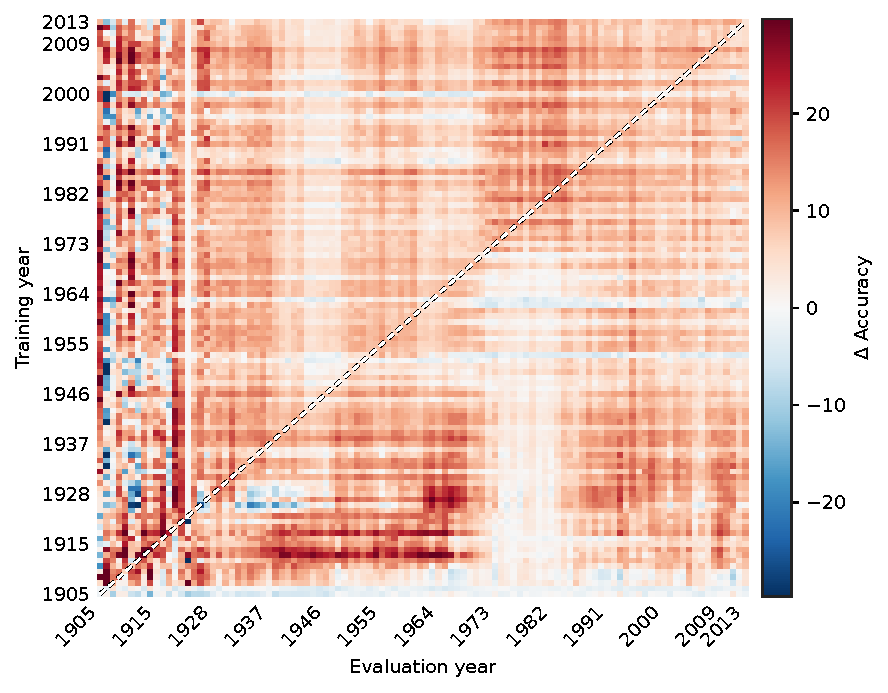
\includegraphics[width=0.49\linewidth]{plots_experiments/yearbook/deviation/CNN-S_deviation.pdf}
    \caption{CNN-S}
    \label{fig:yearbook_CNN_S}
\end{subfigure}
\hfill
\begin{subfigure}[t]{0.49\textwidth}\centering
    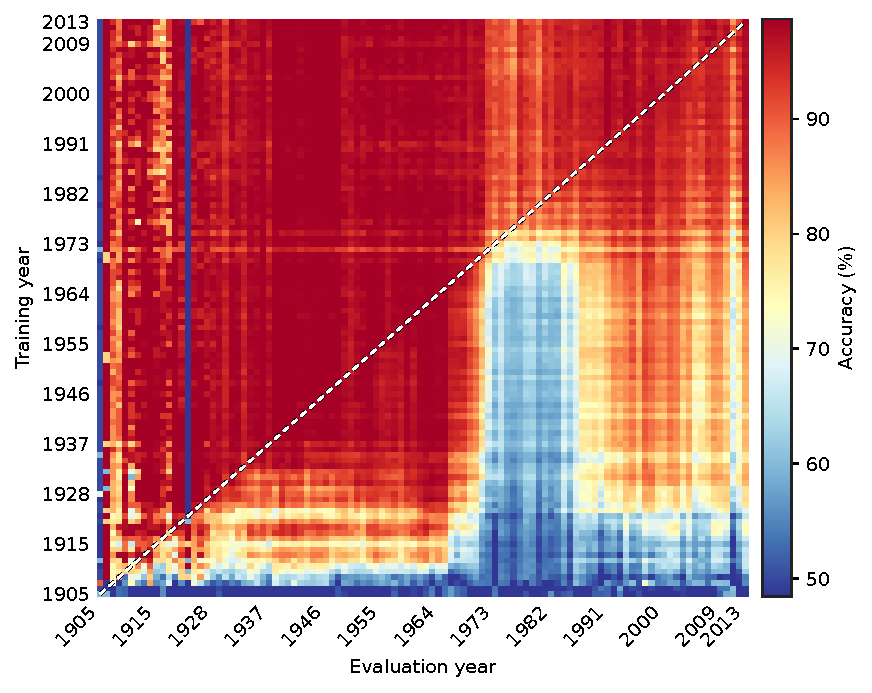
\includegraphics[width=0.49\linewidth]{plots_experiments/yearbook/raw/CNN-M_drift_matrix.pdf}\hfill
    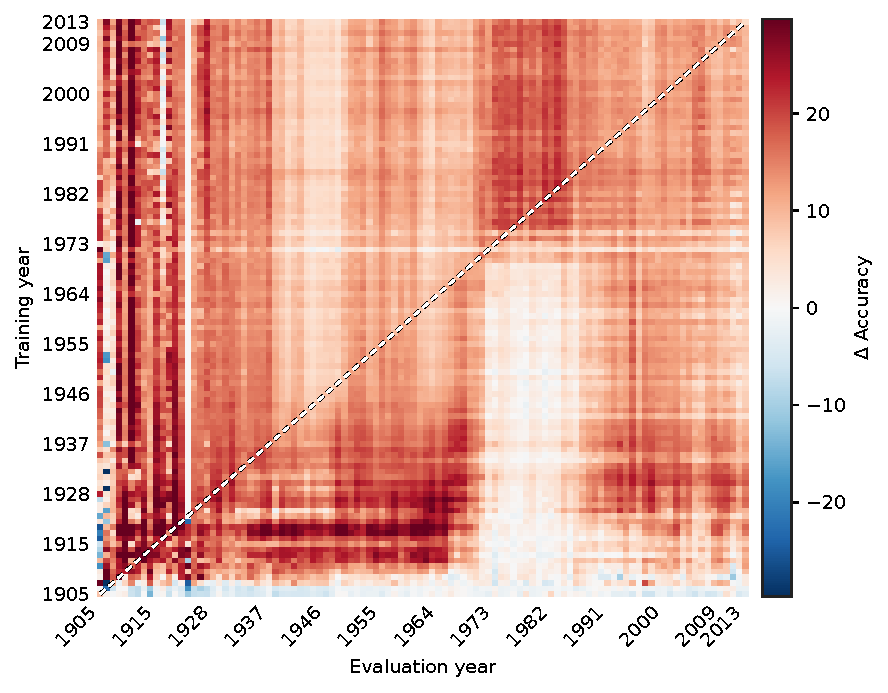
\includegraphics[width=0.49\linewidth]{plots_experiments/yearbook/deviation/CNN-M_deviation.pdf}
    \caption{CNN-M}
    \label{fig:yearbook_CNN_M}
\end{subfigure}

\begin{subfigure}[t]{0.49\textwidth}\centering
    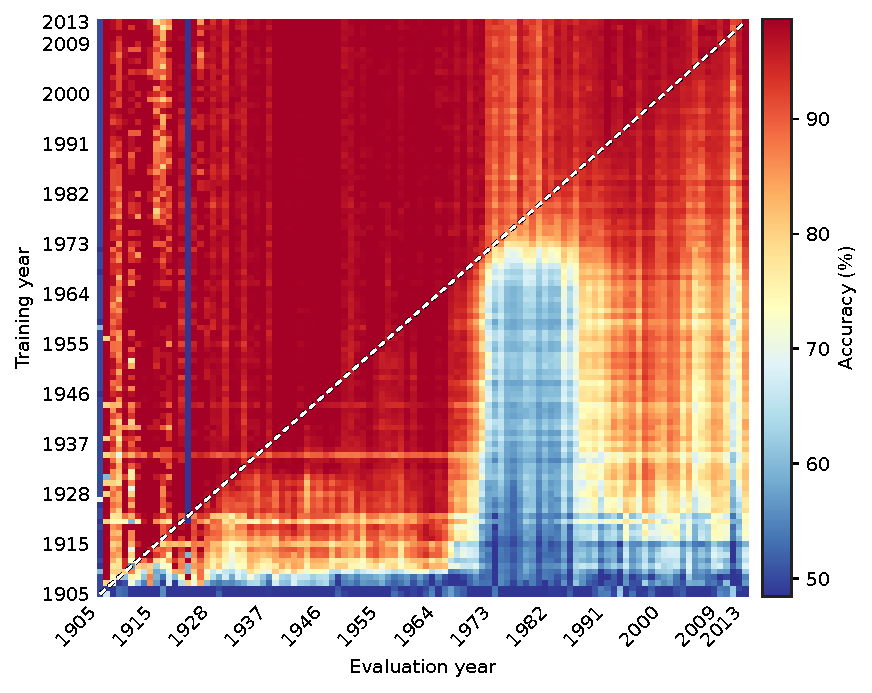
\includegraphics[width=0.49\linewidth]{plots_experiments/yearbook/raw/CNN-L_drift_matrix.pdf}\hfill
    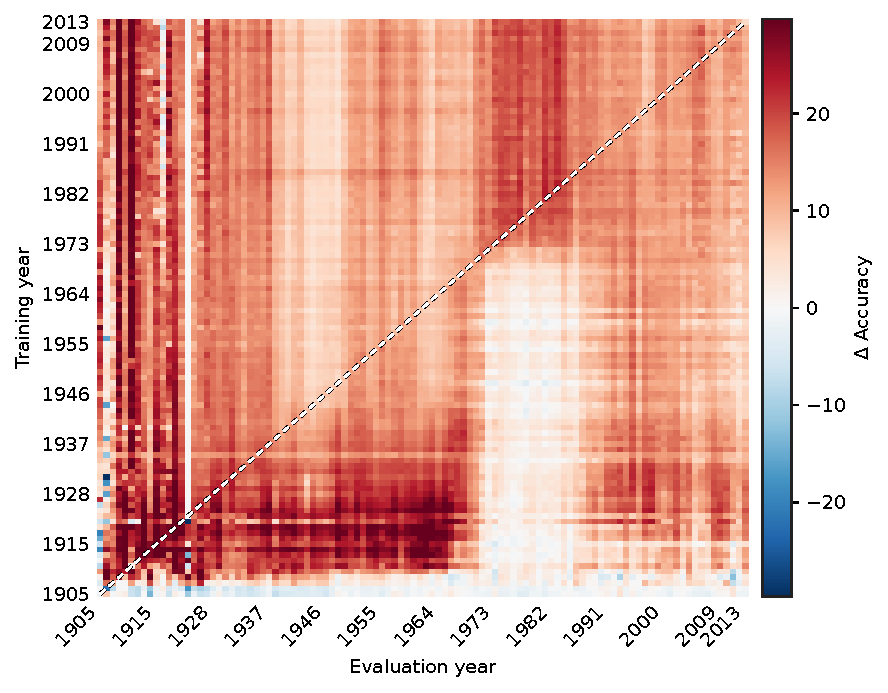
\includegraphics[width=0.49\linewidth]{plots_experiments/yearbook/deviation/CNN-L_deviation.pdf}
    \caption{CNN-L}
    \label{fig:yearbook_CNN_L}
\end{subfigure}
\caption{CNN models: Accuracy drift matrix $M^{(m)}$ and deviation from the cohort mean $\Delta^{(m)} = M^{(m)} - \bar{M}$ for each model, shown on a sequential and a zero-centred diverging scale, respectively.}
\label{fig:yearbook_family_image_cnn}
\end{figure}

\subsection{ResNet}

\begin{figure}[H]
\centering
\begin{subfigure}[t]{0.49\textwidth}\centering
    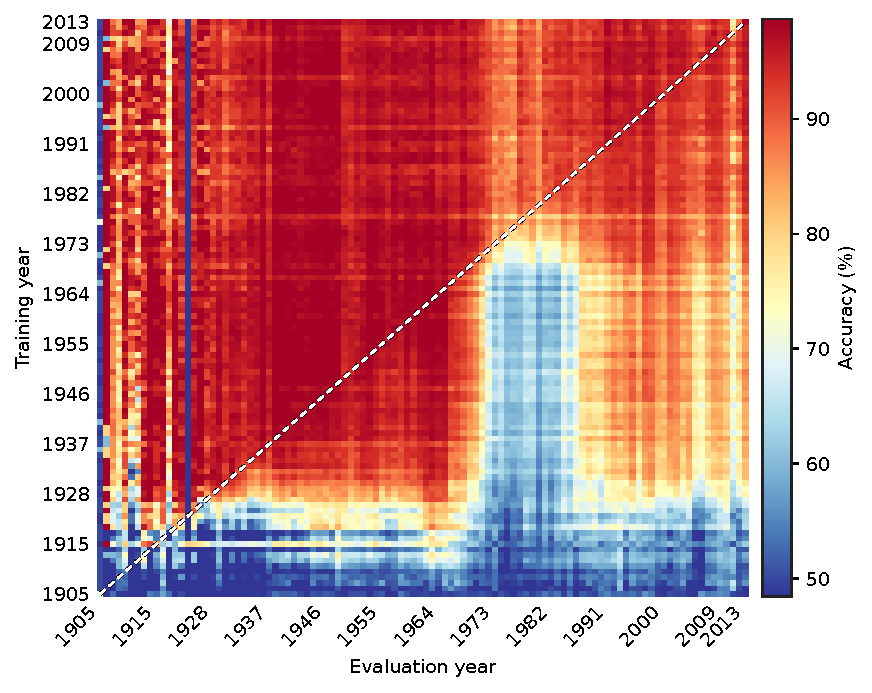
\includegraphics[width=0.49\linewidth]{plots_experiments/yearbook/raw/ResNet-S_drift_matrix.pdf}\hfill
    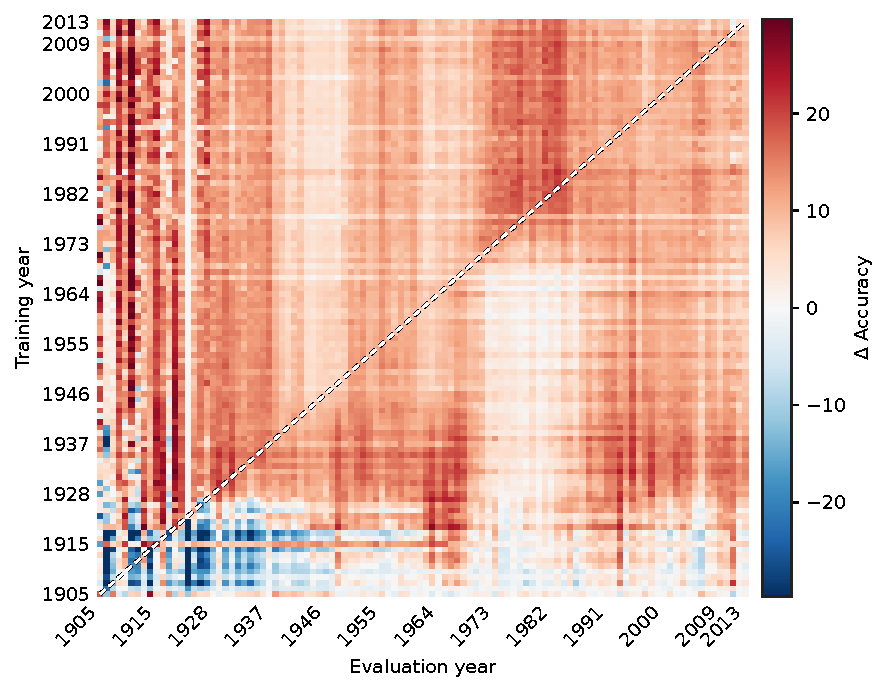
\includegraphics[width=0.49\linewidth]{plots_experiments/yearbook/deviation/ResNet-S_deviation.pdf}
    \caption{ResNet-S}
    \label{fig:yearbook_ResNet_S}
\end{subfigure}
\hfill
\begin{subfigure}[t]{0.49\textwidth}\centering
    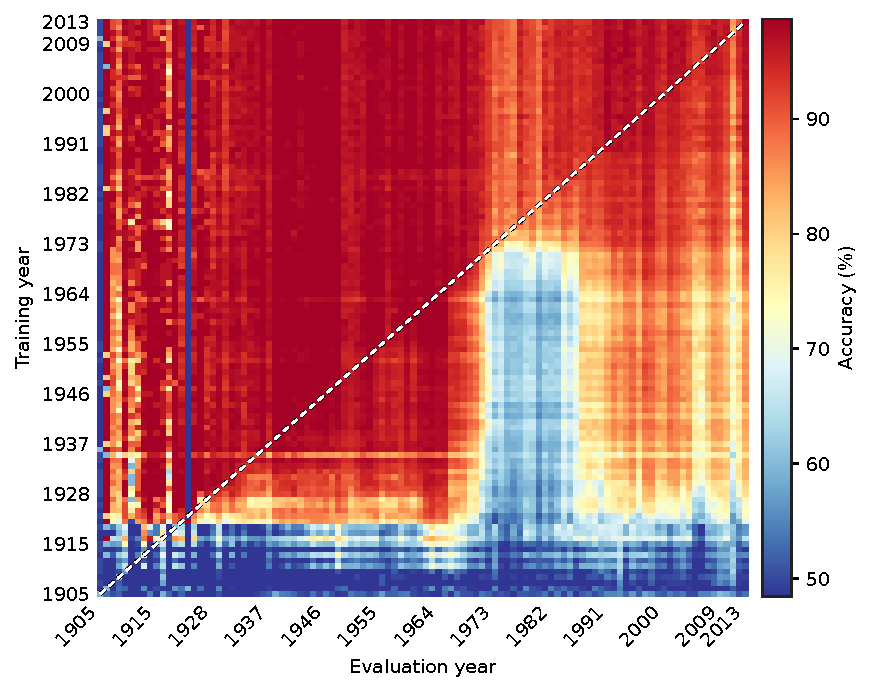
\includegraphics[width=0.49\linewidth]{plots_experiments/yearbook/raw/ResNet-M_drift_matrix.pdf}\hfill
    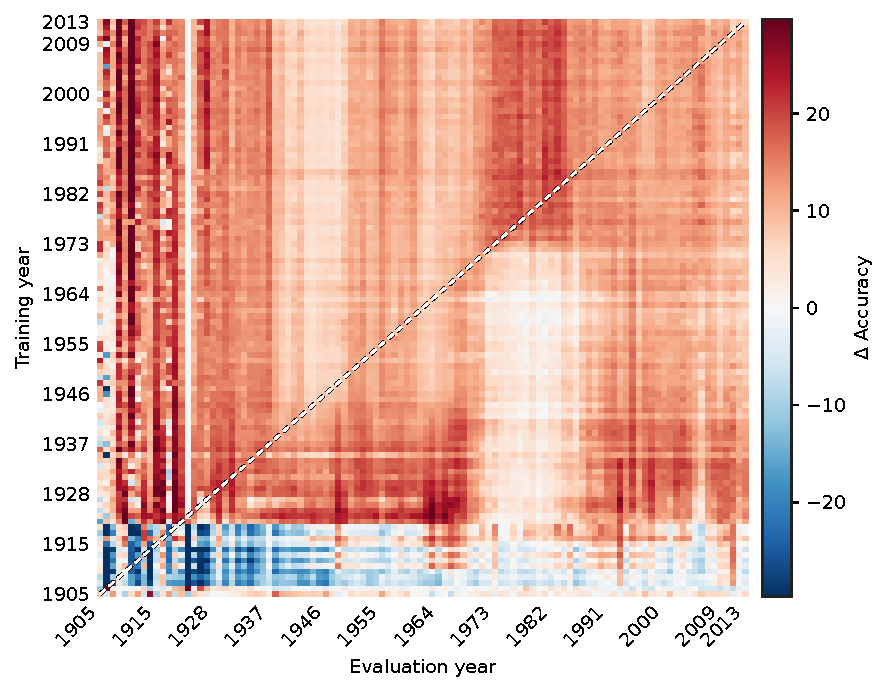
\includegraphics[width=0.49\linewidth]{plots_experiments/yearbook/deviation/ResNet-M_deviation.pdf}
    \caption{ResNet-M}
    \label{fig:yearbook_ResNet_M}
\end{subfigure}

\begin{subfigure}[t]{0.49\textwidth}\centering
    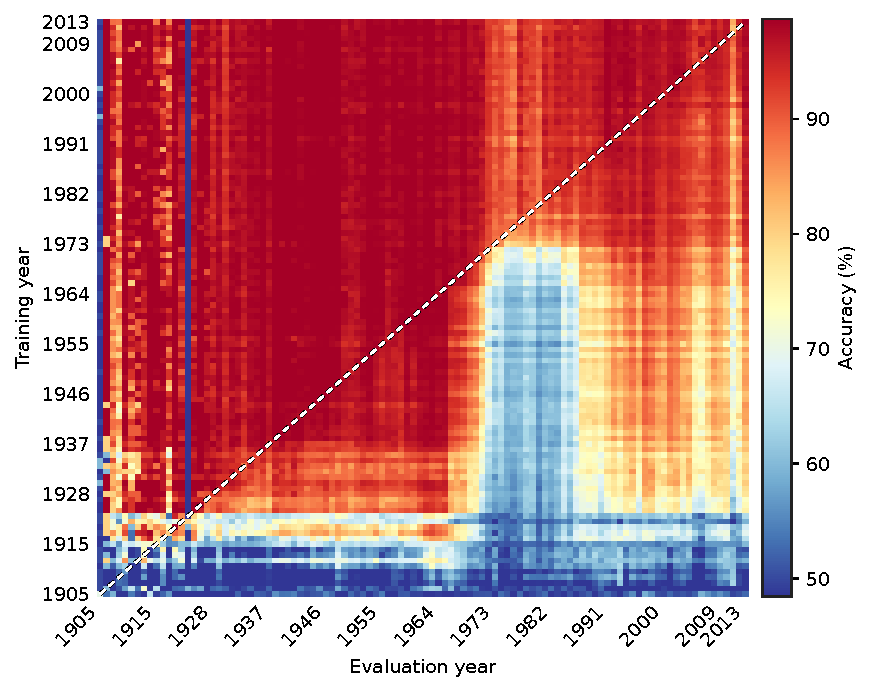
\includegraphics[width=0.49\linewidth]{plots_experiments/yearbook/raw/ResNet-L_drift_matrix.pdf}\hfill
    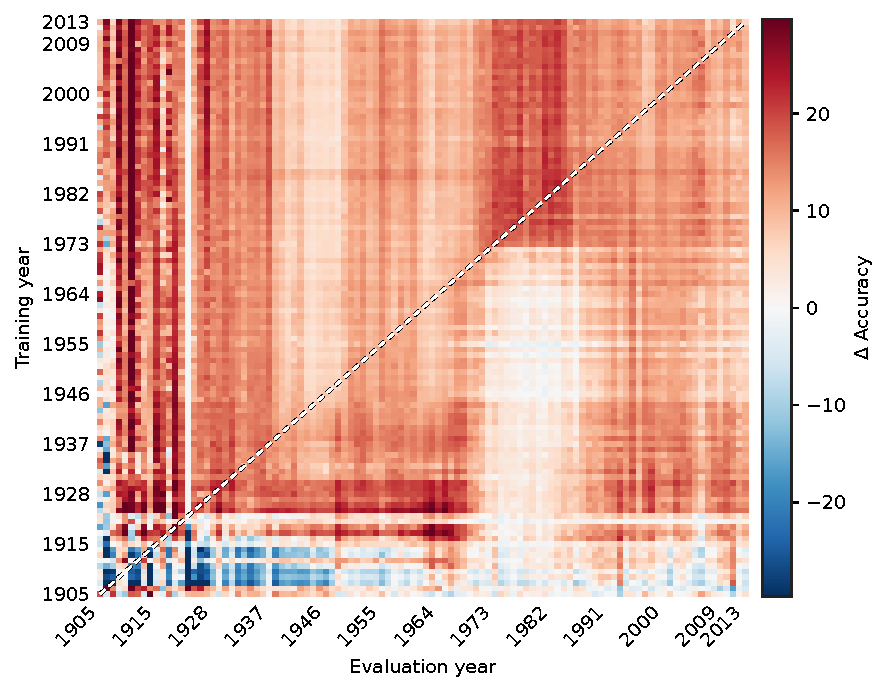
\includegraphics[width=0.49\linewidth]{plots_experiments/yearbook/deviation/ResNet-L_deviation.pdf}
    \caption{ResNet-L}
    \label{fig:yearbook_ResNet_L}
\end{subfigure}
\caption{ResNet models: Accuracy drift matrix $M^{(m)}$ and deviation from the cohort mean $\Delta^{(m)} = M^{(m)} - \bar{M}$ for each model, shown on a sequential and a zero-centred diverging scale, respectively.}
\label{fig:yearbook_family_image_resnet}
\end{figure}

\subsection{ViT}

\begin{figure}[H]
\centering
\begin{subfigure}[t]{0.49\textwidth}\centering
    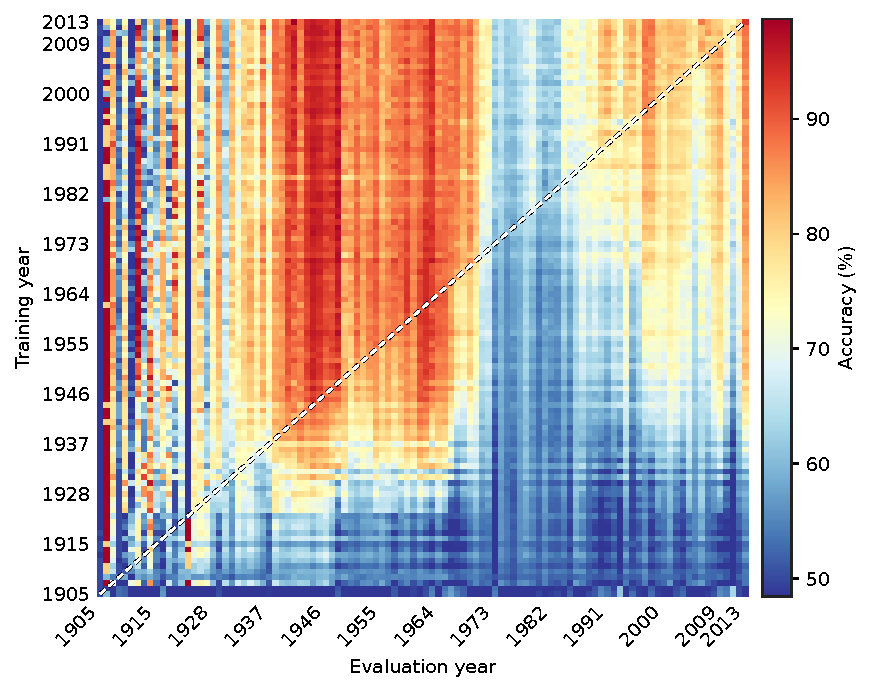
\includegraphics[width=0.49\linewidth]{plots_experiments/yearbook/raw/ViT-S_drift_matrix.pdf}\hfill
    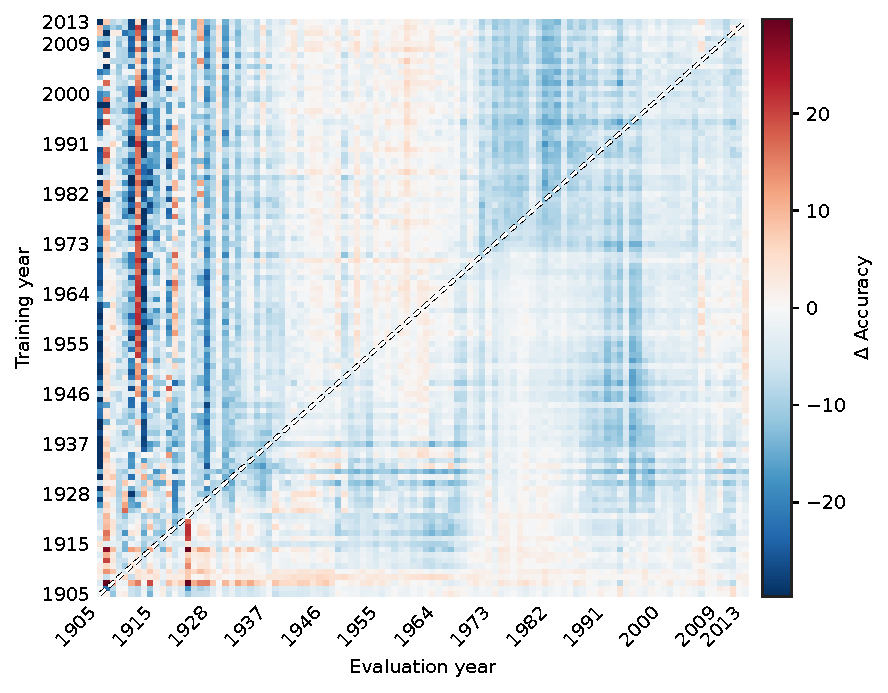
\includegraphics[width=0.49\linewidth]{plots_experiments/yearbook/deviation/ViT-S_deviation.pdf}
    \caption{ViT-S}
    \label{fig:yearbook_ViT_S}
\end{subfigure}
\hfill
\begin{subfigure}[t]{0.49\textwidth}\centering
    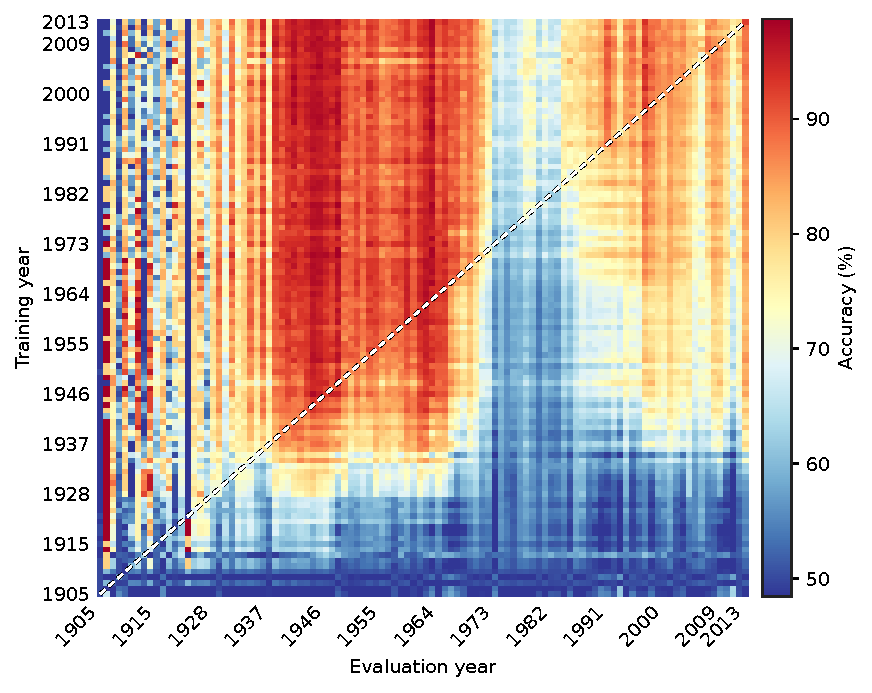
\includegraphics[width=0.49\linewidth]{plots_experiments/yearbook/raw/ViT-M_drift_matrix.pdf}\hfill
    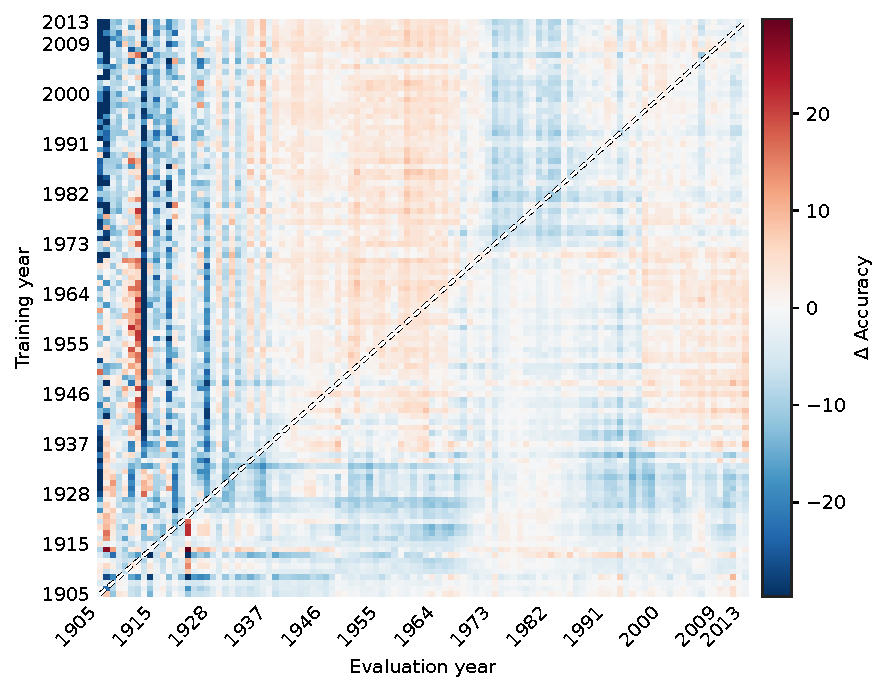
\includegraphics[width=0.49\linewidth]{plots_experiments/yearbook/deviation/ViT-M_deviation.pdf}
    \caption{ViT-M}
    \label{fig:yearbook_ViT_M}
\end{subfigure}

\begin{subfigure}[t]{0.49\textwidth}\centering
    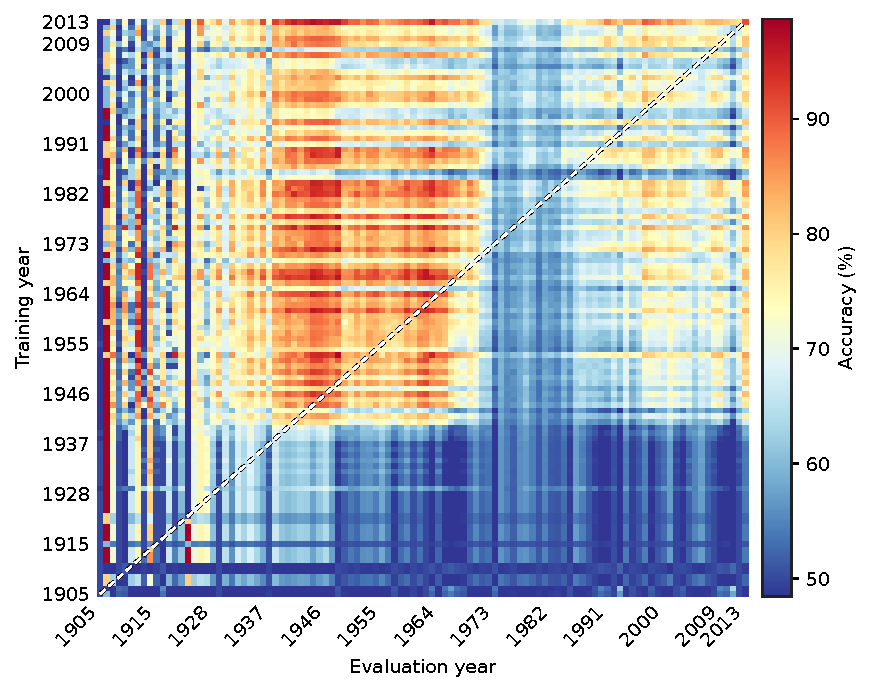
\includegraphics[width=0.49\linewidth]{plots_experiments/yearbook/raw/ViT-L_drift_matrix.pdf}\hfill
    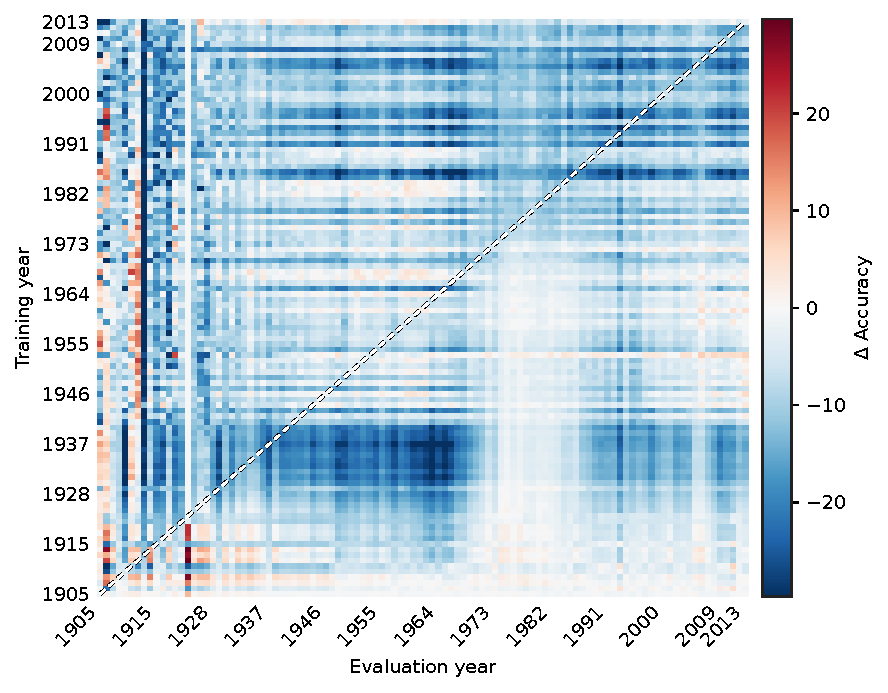
\includegraphics[width=0.49\linewidth]{plots_experiments/yearbook/deviation/ViT-L_deviation.pdf}
    \caption{ViT-L}
    \label{fig:yearbook_ViT_L}
\end{subfigure}
\caption{ViT models: Accuracy drift matrix $M^{(m)}$ and deviation from the cohort mean $\Delta^{(m)} = M^{(m)} - \bar{M}$ for each model, shown on a sequential and a zero-centred diverging scale, respectively.}
\label{fig:yearbook_family_image_vit}
\end{figure}

\subsection{Transfer}

\begin{figure}[H]
\centering
\begin{subfigure}[t]{0.49\textwidth}\centering
    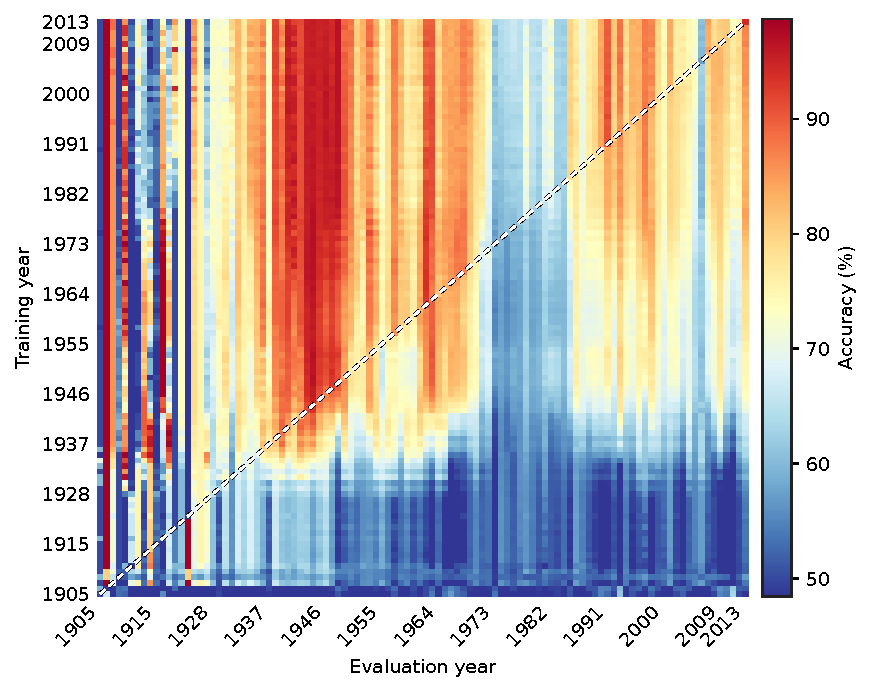
\includegraphics[width=0.49\linewidth]{plots_experiments/yearbook/raw/CLIP-B32_drift_matrix.pdf}\hfill
    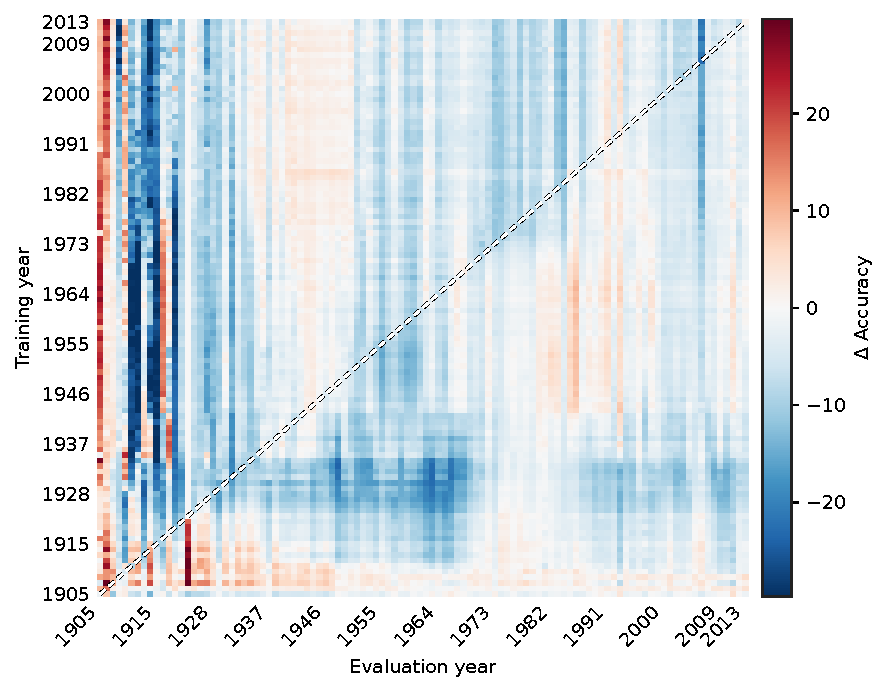
\includegraphics[width=0.49\linewidth]{plots_experiments/yearbook/deviation/CLIP-B32_deviation.pdf}
    \caption{CLIP-B32}
    \label{fig:yearbook_CLIP_B32}
\end{subfigure}
\hfill
\begin{subfigure}[t]{0.49\textwidth}\centering
    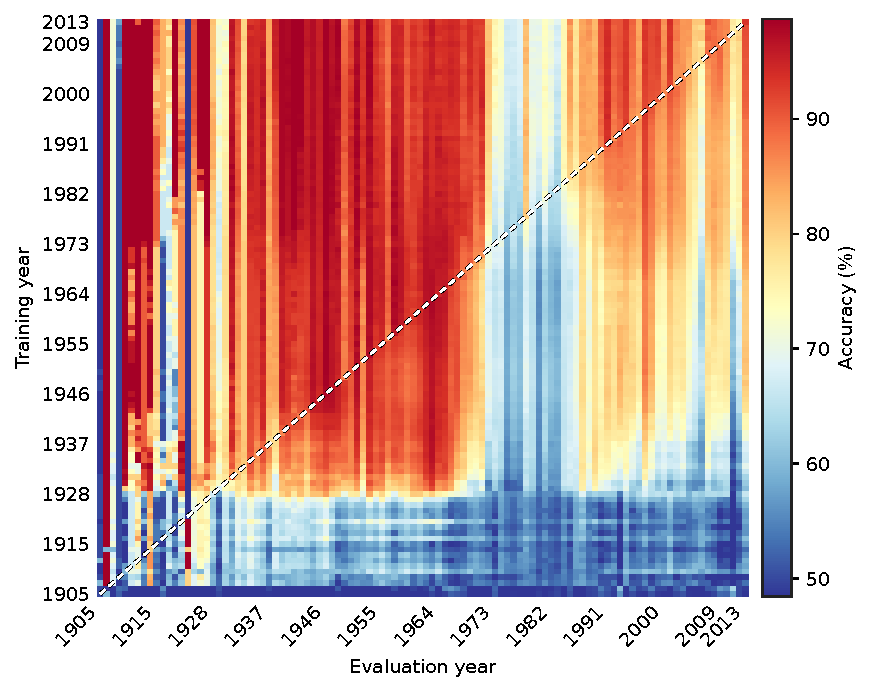
\includegraphics[width=0.49\linewidth]{plots_experiments/yearbook/raw/ConvNeXt-S_drift_matrix.pdf}\hfill
    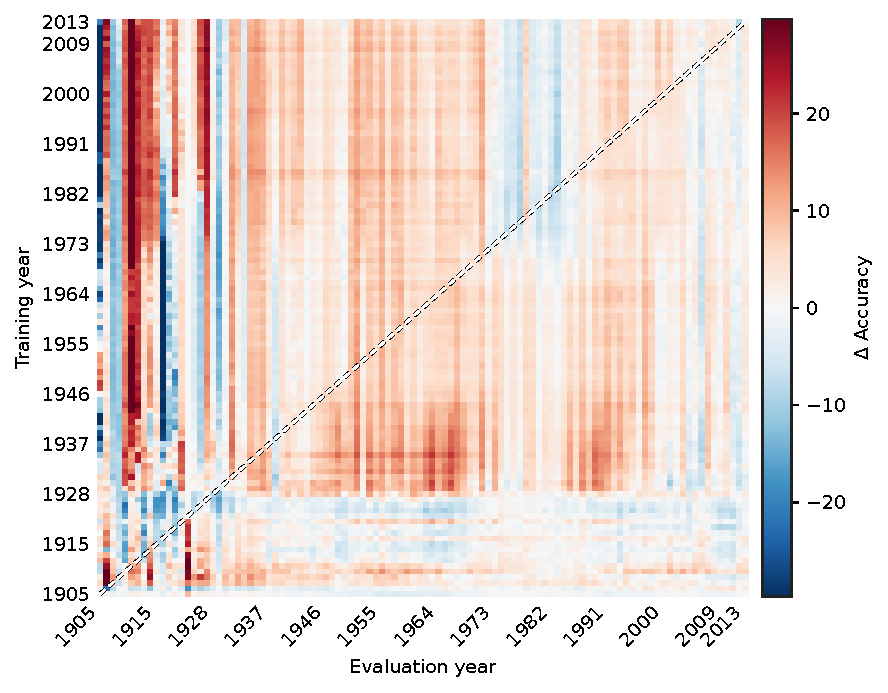
\includegraphics[width=0.49\linewidth]{plots_experiments/yearbook/deviation/ConvNeXt-S_deviation.pdf}
    \caption{ConvNeXt-S}
    \label{fig:yearbook_ConvNeXt_S}
\end{subfigure}

\begin{subfigure}[t]{0.49\textwidth}\centering
    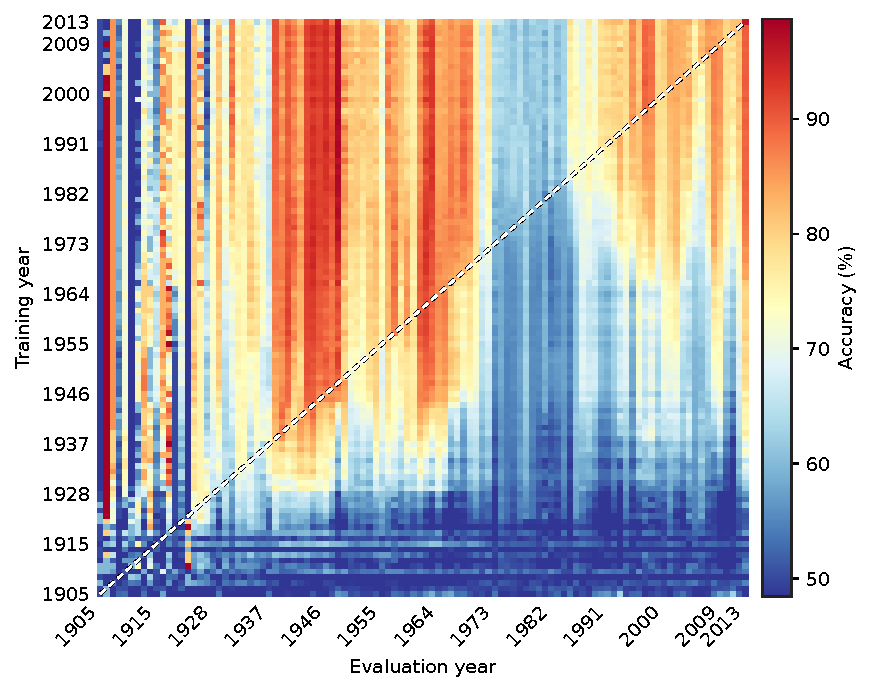
\includegraphics[width=0.49\linewidth]{plots_experiments/yearbook/raw/DINOv2-S_drift_matrix.pdf}\hfill
    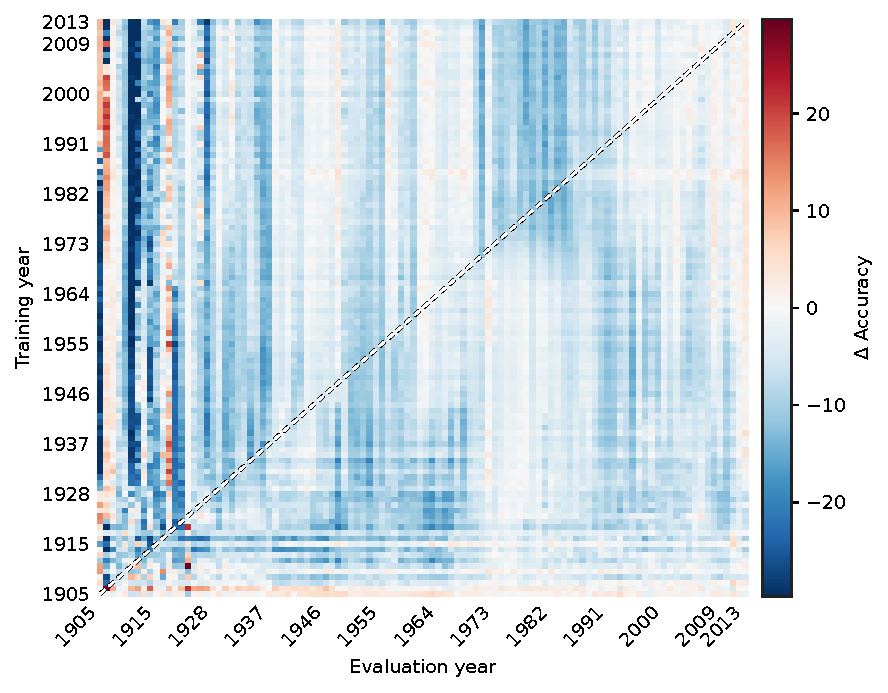
\includegraphics[width=0.49\linewidth]{plots_experiments/yearbook/deviation/DINOv2-S_deviation.pdf}
    \caption{DINOv2-S}
    \label{fig:yearbook_DINOv2_S}
\end{subfigure}
\hfill
\begin{subfigure}[t]{0.49\textwidth}\centering
    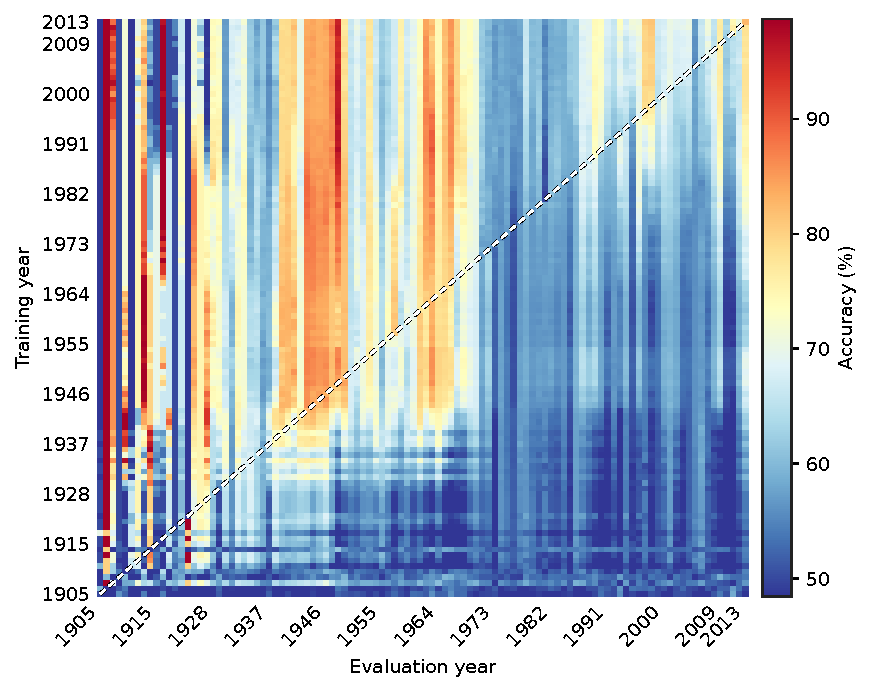
\includegraphics[width=0.49\linewidth]{plots_experiments/yearbook/raw/DINOv3-S_drift_matrix.pdf}\hfill
    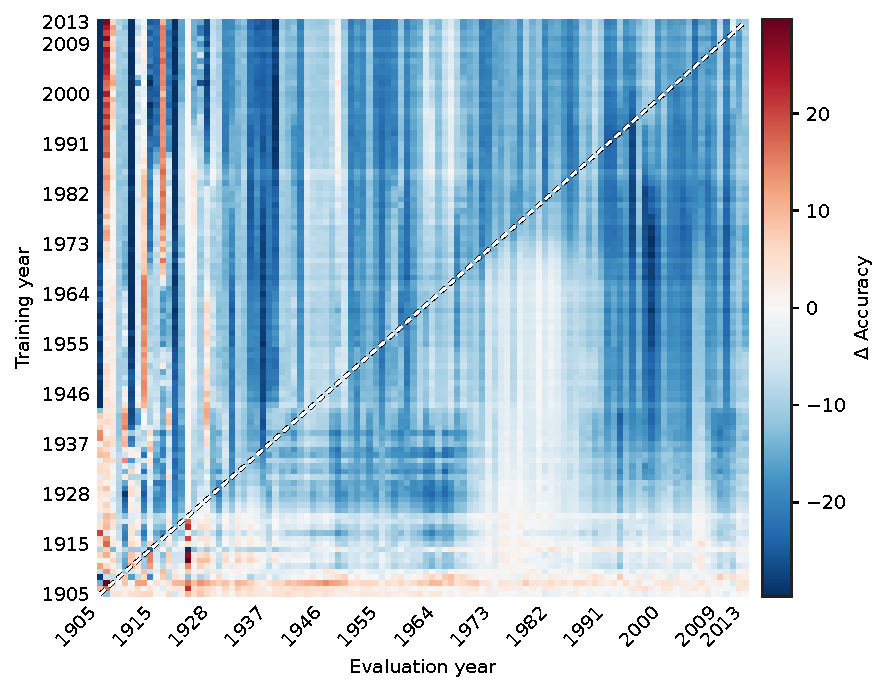
\includegraphics[width=0.49\linewidth]{plots_experiments/yearbook/deviation/DINOv3-S_deviation.pdf}
    \caption{DINOv3-S}
    \label{fig:yearbook_DINOv3_S}
\end{subfigure}

\begin{subfigure}[t]{0.49\textwidth}\centering
    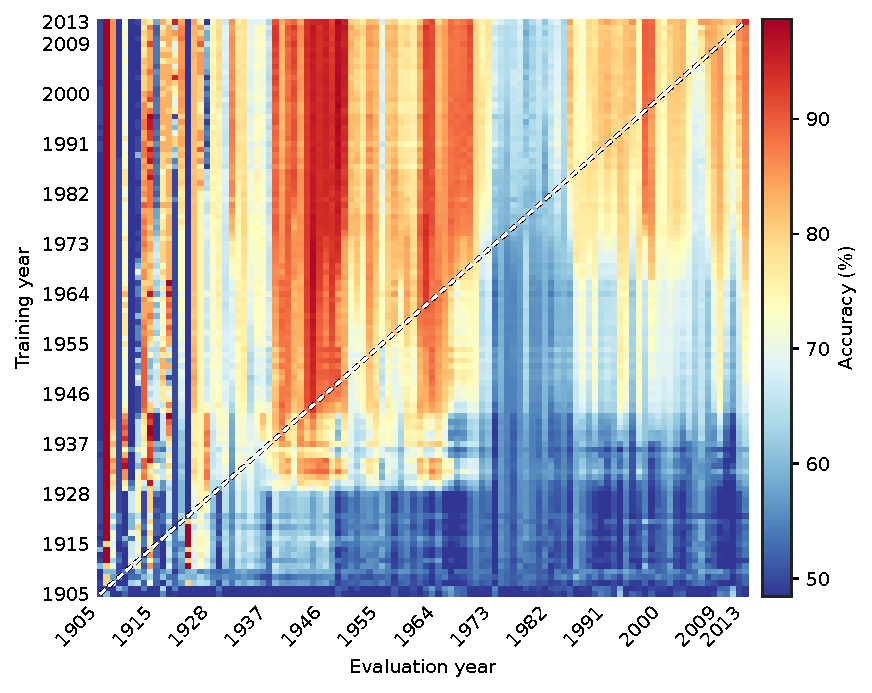
\includegraphics[width=0.49\linewidth]{plots_experiments/yearbook/raw/EVA02-B_drift_matrix.pdf}\hfill
    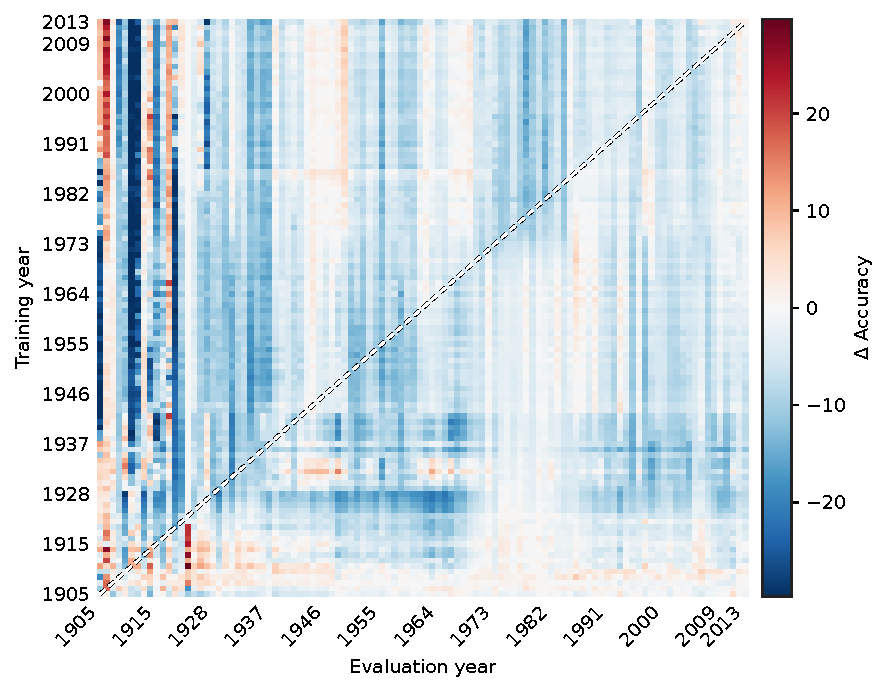
\includegraphics[width=0.49\linewidth]{plots_experiments/yearbook/deviation/EVA02-B_deviation.pdf}
    \caption{EVA02-B}
    \label{fig:yearbook_EVA02_B}
\end{subfigure}
\hfill
\begin{subfigure}[t]{0.49\textwidth}\centering
    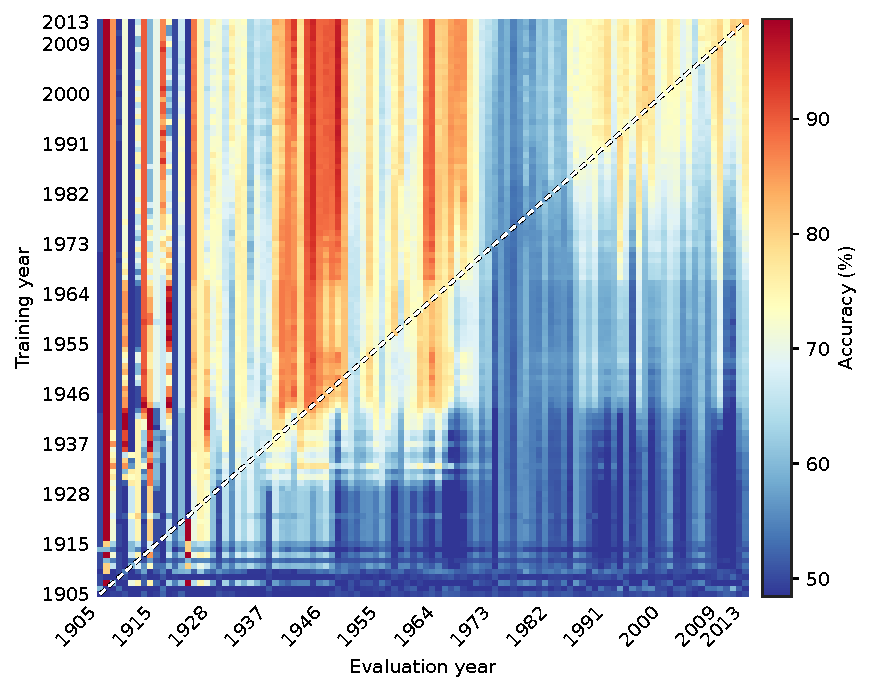
\includegraphics[width=0.49\linewidth]{plots_experiments/yearbook/raw/MAE-B_drift_matrix.pdf}\hfill
    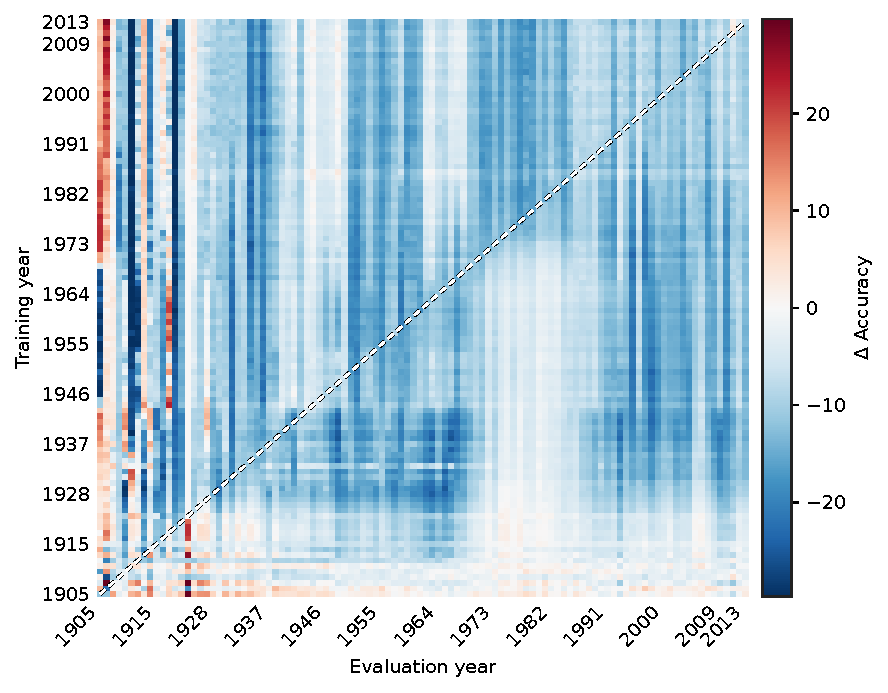
\includegraphics[width=0.49\linewidth]{plots_experiments/yearbook/deviation/MAE-B_deviation.pdf}
    \caption{MAE-B}
    \label{fig:yearbook_MAE_B}
\end{subfigure}

\begin{subfigure}[t]{0.49\textwidth}\centering
    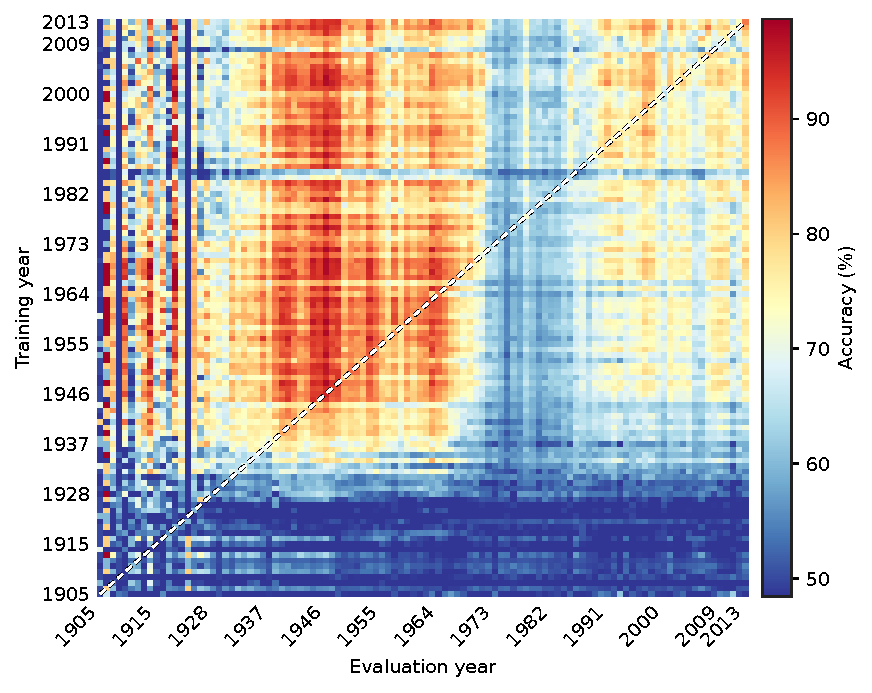
\includegraphics[width=0.49\linewidth]{plots_experiments/yearbook/raw/ResNet50-IN_drift_matrix.pdf}\hfill
    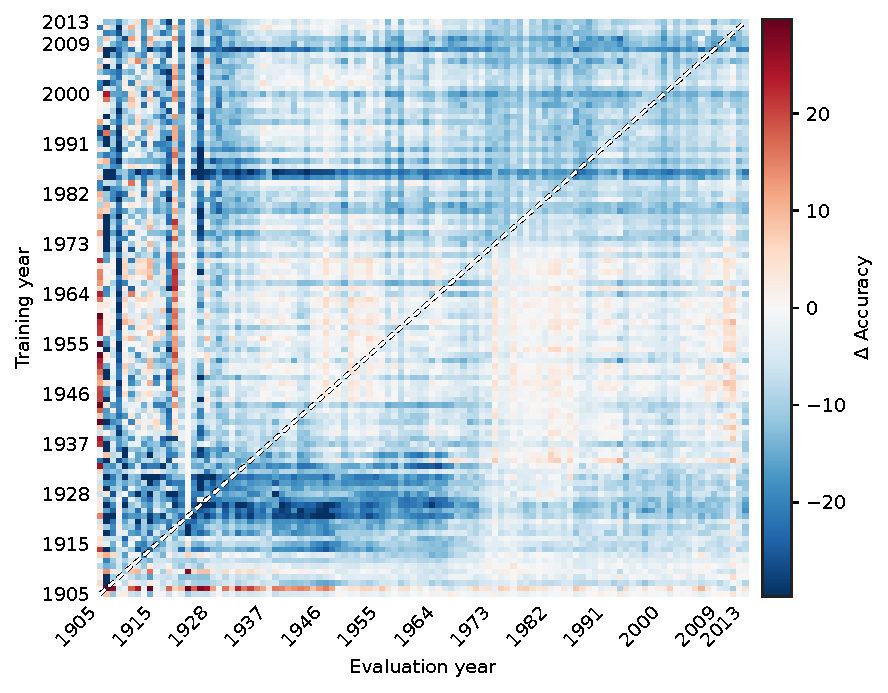
\includegraphics[width=0.49\linewidth]{plots_experiments/yearbook/deviation/ResNet50-IN_deviation.pdf}
    \caption{ResNet50-IN}
    \label{fig:yearbook_ResNet50_IN}
\end{subfigure}
\hfill
\begin{subfigure}[t]{0.49\textwidth}\centering
    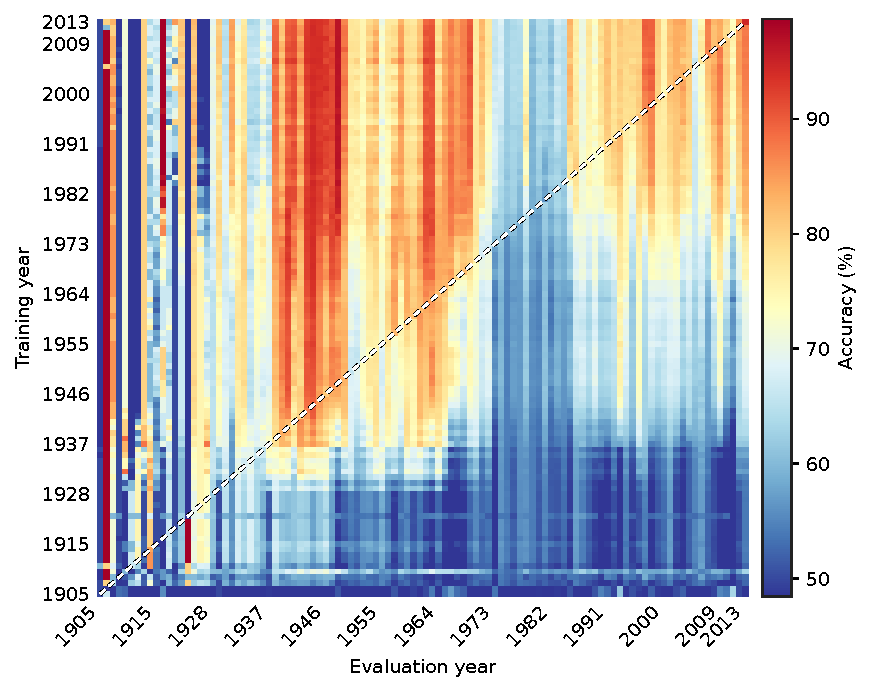
\includegraphics[width=0.49\linewidth]{plots_experiments/yearbook/raw/SigLIP-B_drift_matrix.pdf}\hfill
    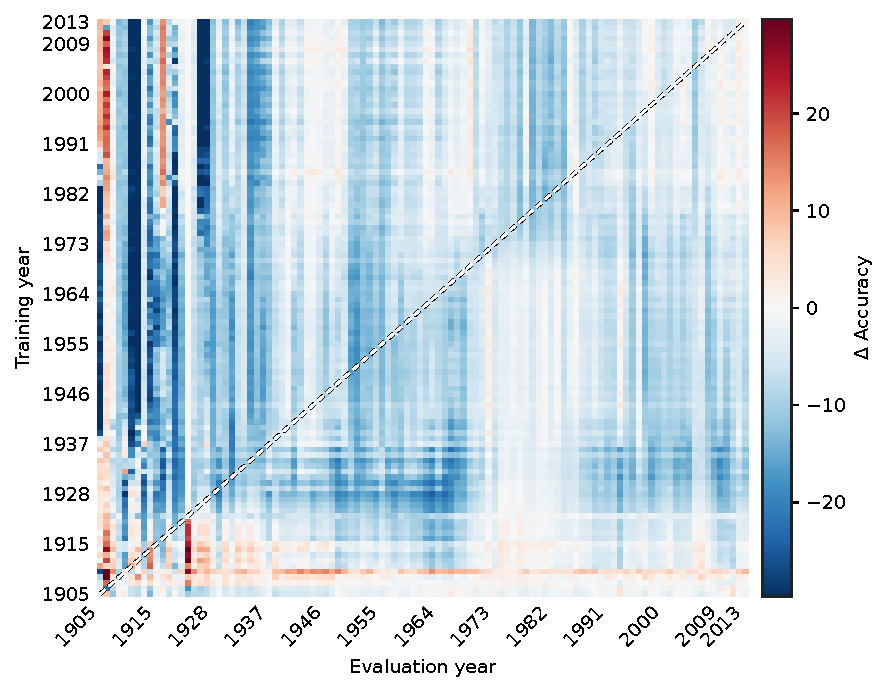
\includegraphics[width=0.49\linewidth]{plots_experiments/yearbook/deviation/SigLIP-B_deviation.pdf}
    \caption{SigLIP-B}
    \label{fig:yearbook_SigLIP_B}
\end{subfigure}

\begin{subfigure}[t]{0.49\textwidth}\centering
    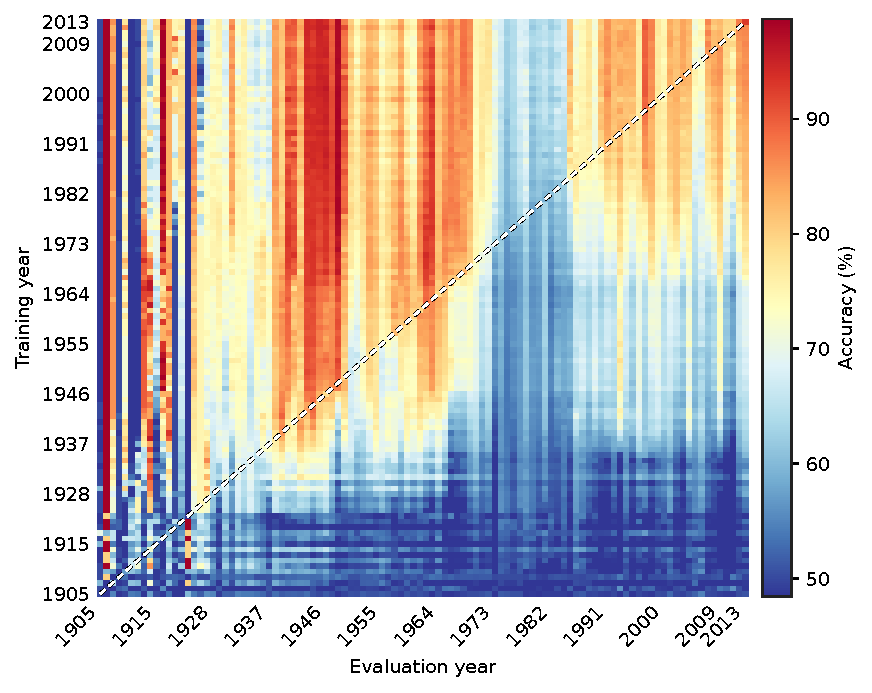
\includegraphics[width=0.49\linewidth]{plots_experiments/yearbook/raw/ViT-S16-IN21k_drift_matrix.pdf}\hfill
    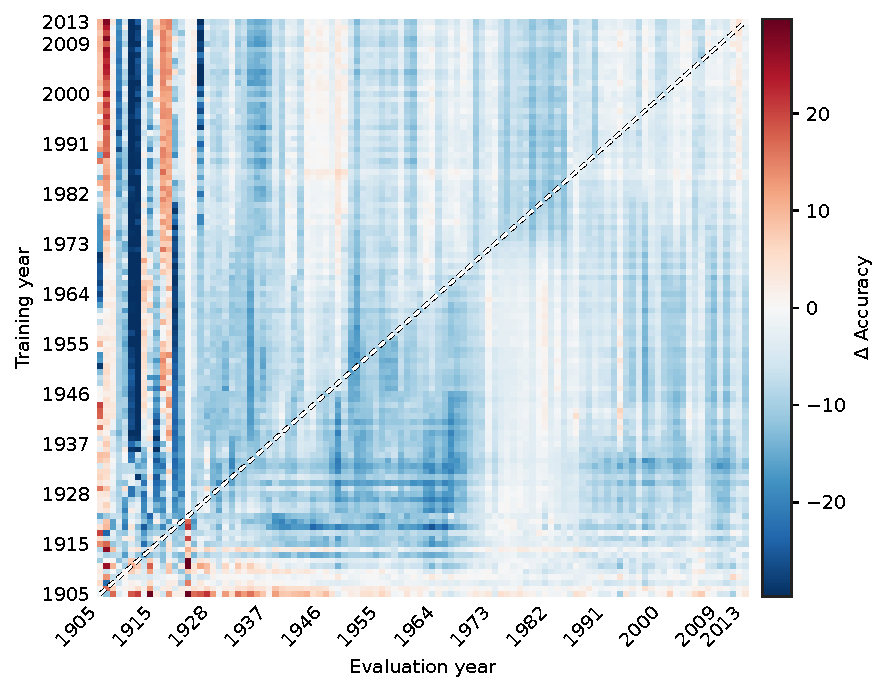
\includegraphics[width=0.49\linewidth]{plots_experiments/yearbook/deviation/ViT-S16-IN21k_deviation.pdf}
    \caption{ViT-S16-IN21k}
    \label{fig:yearbook_ViT_S16_IN21k}
\end{subfigure}
\caption{Transfer models: Accuracy drift matrix $M^{(m)}$ and deviation from the cohort mean $\Delta^{(m)} = M^{(m)} - \bar{M}$ for each model, shown on a sequential and a zero-centred diverging scale, respectively.}
\label{fig:yearbook_family_image_transfer}
\end{figure}

\subsection{Forgetting and Rankings}
\label{app:yearbook_forgetting}

\noindent To see how quickly each model forgets, we summarize its drift matrix as a forgetting curve. The curve plots the Accuracy against the lag $\ell = j - i$, the number of slices between the training cutoff $i$ and the evaluation slice $j$. At each lag we average over all training cutoffs,
\[ F(\ell) = \operatorname{mean}_{i} M_{i,\,i+\ell}. \]
The result is the Accuracy at a fixed temporal distance, independent of which period a model was trained on. This separates the effect of temporal distance from the difficulty of any single slice.

\begin{figure}[H]
\centering
\begin{subfigure}[t]{0.49\textwidth}\centering
    
\includegraphics[width=\linewidth]{plots_experiments/yearbook/forgetting.pdf}
    \caption{Per model}
    \label{fig:yearbook_forgetting}
\end{subfigure}\hfill
\begin{subfigure}[t]{0.49\textwidth}\centering
    
\includegraphics[width=\linewidth]{plots_experiments/yearbook/forgetting_by_family.pdf}
    \caption{Per model family}
    \label{fig:yearbook_forgetting_family}
\end{subfigure}
\caption{Forgetting curves: each model (left) and averaged within each family (right).}
\label{fig:yearbook_forgetting_combined}
\end{figure}

\begin{figure}[H]
\centering
\begin{subfigure}[t]{0.49\textwidth}\centering
    
\includegraphics[width=\linewidth]{plots_experiments/yearbook/ranking_future_performance.pdf}
    \caption{By future performance}
    \label{fig:yearbook_ranking_future}
\end{subfigure}\hfill
\begin{subfigure}[t]{0.49\textwidth}\centering
    
\includegraphics[width=\linewidth]{plots_experiments/yearbook/ranking_decay.pdf}
    \caption{By decay}
    \label{fig:yearbook_ranking_decay}
\end{subfigure}
\caption{Models ranked by mean future performance and by temporal decay.}
\label{fig:yearbook_rankings}
\end{figure}

\subsection{Result Tables}

\begin{table}[H]
\centering
\footnotesize
\caption{Temporal robustness on Yearbook.}
\label{tab:robustness_yearbook}
\begin{minipage}[t]{0.49\linewidth}
\centering
\resizebox{\ifdim\width>\linewidth \linewidth\else\width\fi}{!}{%
\begin{tabular}{l rr}
\toprule
Model & Future (\%) & Decay (\%) \\
\midrule
MLP-S & 62.3 & 7.1 \\
DINOv3-S & 57.9 & 7.9 \\
ViT-L & 60.3 & 8.0 \\
MAE-B & 59.0 & 8.4 \\
ResNet50-IN & 61.9 & 8.7 \\
CLIP-B32 & 64.1 & 9.1 \\
SigLIP-B & 62.4 & 9.2 \\
ConvNeXt-S & 70.6 & 9.2 \\
EVA02-B & 63.4 & 9.3 \\
ViT-S & 64.6 & 9.6 \\
DINOv2-S & 62.7 & 9.8 \\
\bottomrule
\end{tabular}}
\end{minipage}\hfill
\begin{minipage}[t]{0.49\linewidth}
\centering
\resizebox{\ifdim\width>\linewidth \linewidth\else\width\fi}{!}{%
\begin{tabular}{l rr}
\toprule
Model & Future (\%) & Decay (\%) \\
\midrule
ViT-M & 66.1 & 10.1 \\
ViT-S16-IN21k & 61.8 & 10.4 \\
MLP-L & 72.7 & 12.2 \\
ResNet-S & 75.0 & 12.3 \\
CNN-S & 74.7 & 12.3 \\
MLP-M & 73.0 & 12.7 \\
ResNet-M & 75.8 & 13.1 \\
CNN-L & 79.0 & 13.7 \\
ResNet-L & 76.1 & 13.9 \\
CNN-M & 78.4 & 13.9 \\
\bottomrule
\end{tabular}}
\end{minipage}
\end{table}


\noindent
\begin{minipage}[t]{0.49\linewidth}
\centering
\scriptsize
\setlength{\tabcolsep}{4pt}
\captionof{table}{Yearbook: models trained up to 1905, ordered by future performance.}
\label{tab:yearbook_cutoff_1905}
\resizebox{\ifdim\width>\linewidth \linewidth\else\width\fi}{!}{%
\begin{tabular}{c l rrr}
\toprule
Rank & Model & Accuracy (\%) & Future (\%) & Decay (\%) \\
\midrule
1 & ViT-S16-IN21k & 50.0 & 50.7 & -0.7 \\
2 & ResNet-M & 60.0 & 50.3 & 9.7 \\
3 & ResNet-L & 70.0 & 50.1 & 19.9 \\
4 & MLP-L & 40.0 & 49.8 & -9.8 \\
5 & MAE-B & 40.0 & 49.5 & -9.5 \\
6 & ResNet-S & 70.0 & 49.3 & 20.7 \\
7 & DINOv2-S & 50.0 & 48.5 & 1.5 \\
8 & DINOv3-S & 50.0 & 48.3 & 1.7 \\
9 & ViT-L & 50.0 & 46.8 & 3.2 \\
10 & MLP-S & 40.0 & 46.3 & -6.3 \\
11 & ConvNeXt-S & 50.0 & 46.1 & 3.9 \\
12 & ViT-M & 50.0 & 45.7 & 4.3 \\
13 & CNN-L & 50.0 & 45.4 & 4.6 \\
14 & ViT-S & 50.0 & 45.1 & 4.9 \\
15 & ResNet50-IN & 50.0 & 45.1 & 4.9 \\
16 & EVA02-B & 50.0 & 44.9 & 5.1 \\
17 & MLP-M & 50.0 & 44.9 & 5.1 \\
18 & CNN-S & 50.0 & 44.9 & 5.1 \\
19 & CLIP-B32 & 50.0 & 44.7 & 5.3 \\
20 & CNN-M & 60.0 & 44.7 & 15.3 \\
21 & SigLIP-B & 50.0 & 44.7 & 5.3 \\
\bottomrule
\end{tabular}}
\end{minipage}
\hfill
\begin{minipage}[t]{0.49\linewidth}
\centering
\scriptsize
\setlength{\tabcolsep}{4pt}
\captionof{table}{Yearbook: models trained up to 1944, ordered by future performance.}
\label{tab:yearbook_cutoff_1944}
\resizebox{\ifdim\width>\linewidth \linewidth\else\width\fi}{!}{%
\begin{tabular}{c l rrr}
\toprule
Rank & Model & Accuracy (\%) & Future (\%) & Decay (\%) \\
\midrule
1 & ResNet-L & 98.4 & 82.9 & 15.5 \\
2 & ResNet-M & 98.3 & 81.9 & 16.4 \\
3 & CNN-M & 98.8 & 81.4 & 17.4 \\
4 & ResNet-S & 98.0 & 81.1 & 16.9 \\
5 & CNN-L & 97.1 & 80.2 & 16.8 \\
6 & CNN-S & 95.0 & 79.1 & 15.9 \\
7 & ConvNeXt-S & 96.3 & 78.5 & 17.8 \\
8 & MLP-M & 93.4 & 77.6 & 15.9 \\
9 & MLP-L & 87.9 & 74.6 & 13.3 \\
10 & ViT-M & 92.6 & 71.4 & 21.2 \\
11 & ViT-L & 91.0 & 70.7 & 20.3 \\
12 & ViT-S & 89.4 & 69.9 & 19.5 \\
13 & CLIP-B32 & 94.3 & 69.9 & 24.5 \\
14 & EVA02-B & 93.1 & 67.9 & 25.2 \\
15 & DINOv2-S & 88.5 & 67.1 & 21.5 \\
16 & SigLIP-B & 88.9 & 66.8 & 22.1 \\
17 & ViT-S16-IN21k & 86.4 & 65.0 & 21.4 \\
18 & ResNet50-IN & 80.2 & 64.8 & 15.3 \\
19 & MAE-B & 86.7 & 62.6 & 24.1 \\
20 & DINOv3-S & 82.7 & 62.4 & 20.3 \\
21 & MLP-S & 65.8 & 57.9 & 7.9 \\
\bottomrule
\end{tabular}}
\end{minipage}


\vspace{1.5ex}

\noindent
\begin{minipage}[t]{0.49\linewidth}
\centering
\scriptsize
\setlength{\tabcolsep}{4pt}
\captionof{table}{Yearbook: models trained up to 1978, ordered by future performance.}
\label{tab:yearbook_cutoff_1978}
\resizebox{\ifdim\width>\linewidth \linewidth\else\width\fi}{!}{%
\begin{tabular}{c l rrr}
\toprule
Rank & Model & Accuracy (\%) & Future (\%) & Decay (\%) \\
\midrule
1 & CNN-L & 85.9 & 91.4 & -5.4 \\
2 & ResNet-M & 88.7 & 90.4 & -1.6 \\
3 & ResNet-L & 87.6 & 89.3 & -1.7 \\
4 & CNN-M & 86.8 & 88.8 & -2.0 \\
5 & MLP-M & 79.4 & 84.5 & -5.1 \\
6 & ResNet-S & 83.4 & 84.4 & -1.0 \\
7 & MLP-L & 75.5 & 83.2 & -7.7 \\
8 & CNN-S & 72.7 & 81.1 & -8.5 \\
9 & ConvNeXt-S & 80.6 & 78.6 & 1.9 \\
10 & ViT-M & 72.4 & 76.8 & -4.4 \\
11 & CLIP-B32 & 69.9 & 74.8 & -5.0 \\
12 & EVA02-B & 60.6 & 73.3 & -12.8 \\
13 & ViT-L & 66.8 & 72.4 & -5.6 \\
14 & DINOv2-S & 64.5 & 72.3 & -7.8 \\
15 & ViT-S & 64.2 & 71.8 & -7.6 \\
16 & ViT-S16-IN21k & 66.5 & 70.7 & -4.3 \\
17 & ResNet50-IN & 72.7 & 70.7 & 2.0 \\
18 & SigLIP-B & 64.8 & 69.9 & -5.1 \\
19 & MLP-S & 67.9 & 69.4 & -1.5 \\
20 & MAE-B & 56.1 & 65.0 & -8.9 \\
21 & DINOv3-S & 60.3 & 59.9 & 0.4 \\
\bottomrule
\end{tabular}}
\end{minipage}
\hfill
\begin{minipage}[t]{0.49\linewidth}
\centering
\scriptsize
\setlength{\tabcolsep}{4pt}
\captionof{table}{Yearbook: models trained up to 2012, ordered by future performance.}
\label{tab:yearbook_cutoff_2012}
\resizebox{\ifdim\width>\linewidth \linewidth\else\width\fi}{!}{%
\begin{tabular}{c l rrr}
\toprule
Rank & Model & Accuracy (\%) & Future (\%) & Decay (\%) \\
\midrule
1 & CNN-L & 93.2 & 98.2 & -5.0 \\
2 & CNN-M & 93.2 & 97.7 & -4.6 \\
3 & ResNet-L & 88.9 & 97.5 & -8.5 \\
4 & ResNet-M & 92.6 & 97.0 & -4.3 \\
5 & ResNet-S & 86.8 & 95.4 & -8.5 \\
6 & CNN-S & 83.7 & 93.4 & -9.7 \\
7 & MLP-L & 87.4 & 91.9 & -4.6 \\
8 & MLP-M & 86.3 & 91.7 & -5.4 \\
9 & ConvNeXt-S & 73.7 & 91.2 & -17.5 \\
10 & DINOv2-S & 82.6 & 90.0 & -7.3 \\
11 & ViT-M & 77.9 & 88.1 & -10.2 \\
12 & ViT-S & 80.5 & 88.0 & -7.5 \\
13 & SigLIP-B & 85.8 & 87.5 & -1.7 \\
14 & EVA02-B & 82.1 & 87.4 & -5.3 \\
15 & CLIP-B32 & 74.7 & 86.6 & -11.9 \\
16 & ViT-S16-IN21k & 87.9 & 86.5 & 1.4 \\
17 & ResNet50-IN & 76.8 & 83.8 & -7.0 \\
18 & DINOv3-S & 71.1 & 77.9 & -6.9 \\
19 & MAE-B & 78.4 & 77.4 & 1.0 \\
20 & MLP-S & 70.0 & 76.1 & -6.1 \\
21 & ViT-L & 66.8 & 74.4 & -7.5 \\
\bottomrule
\end{tabular}}
\end{minipage}


\begin{table}[H]
\centering
\footnotesize
\caption{Yearbook: future performance and decay by model family.}
\label{tab:yearbook_by_family}
\begin{tabular}{l rrrrrrrr}
\toprule
 & \multicolumn{2}{c}{1905} & \multicolumn{2}{c}{1944} & \multicolumn{2}{c}{1978} & \multicolumn{2}{c}{2012} \\
Family & Future & Decay & Future & Decay & Future & Decay & Future & Decay \\
\midrule
CNN & 45.0 & 8.3 & 80.3 & 16.7 & 87.1 & -5.3 & 96.4 & -6.4 \\
MLP & 47.0 & -3.7 & 70.0 & 12.4 & 79.0 & -4.8 & 86.6 & -5.3 \\
ResNet & 49.9 & 16.8 & 82.0 & 16.2 & 88.0 & -1.4 & 96.6 & -7.1 \\
Transfer & 46.9 & 1.9 & 67.2 & 21.4 & 70.6 & -4.4 & 85.4 & -6.1 \\
ViT & 45.9 & 4.1 & 70.7 & 20.3 & 73.7 & -5.9 & 83.5 & -8.4 \\
\bottomrule
\end{tabular}
\end{table}

